% -*- root: ../EstadisticaII.tex -*-

\chapter{Regresión}
El objetivo de la regresión es predecir una/s variable/s en función de la/s otra/s.


\section{Regresión lineal}

Observamos dos variables, X e Y , el objetivo es analizar la relación existente entre ambas, de forma que podamos predecir o aproximar el valor de la variable Y a partir del valor de la variable X.

\begin{itemize}
\item La variable Y se llama variable respuesta.
\item La variable X se llama variable regresora o explicativa.
\end{itemize}

Por ejemplo:
\begin{center}
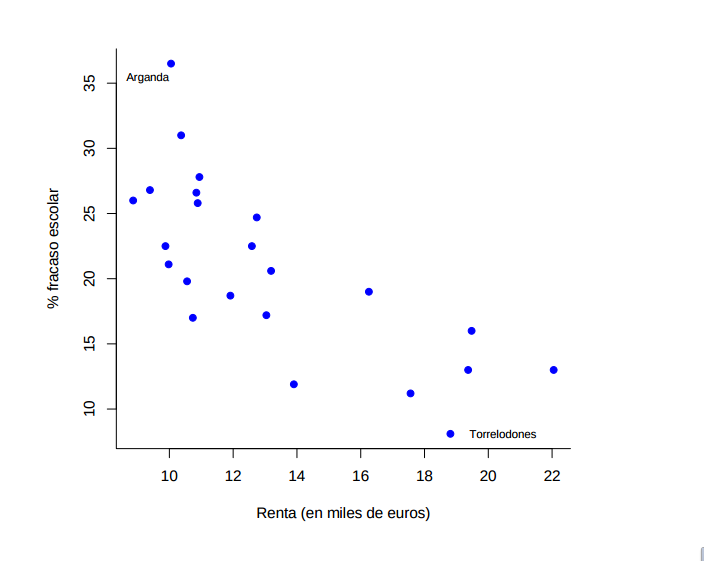
\includegraphics[scale=0.5]{img/RentaVsFracaso.png}
\end{center}

Queremos predecir el fracaso escolar en función de la renta. La variable respuesta es el fracaso escolar, mientras que la variable regresora es la renta.

\subsection{Regresión lineal simple}

Frecuentemente existe una relación lineal entre las variables. En el caso del fracaso escolar,queremos construir una recta $Y_i = β_1 X_i + β_0\; i=1,...,n$ que minimice el error.

El problema es estimar los parámetros $β_0,β_1$. Una manera de hacer esto es:

\subsubsection{Recta de mínimos cuadrados}

\begin{defn}[Recta de mínimos cuadrados]
Estimando $β_i$ por $\hat{β_i}$ obtenemos: \[\hat{Y_i} = \hat{β}_0 + \hat{β}_1 x_i\]

La recta viene dada por los valores $\hat{β}_0, \hat{β}_1$ para los que se minimiza el error cuadrático, es decir:
\[\sum_{i=1}^n \left(Y_i - \hat{Y_i}\right)^2 =  \sum_{i=1}^n \left[ Y_i - (\hat{β}_0 + \hat{β}_1x_i) \right]^2\]
\end{defn}

\begin{example}
\begin{center}
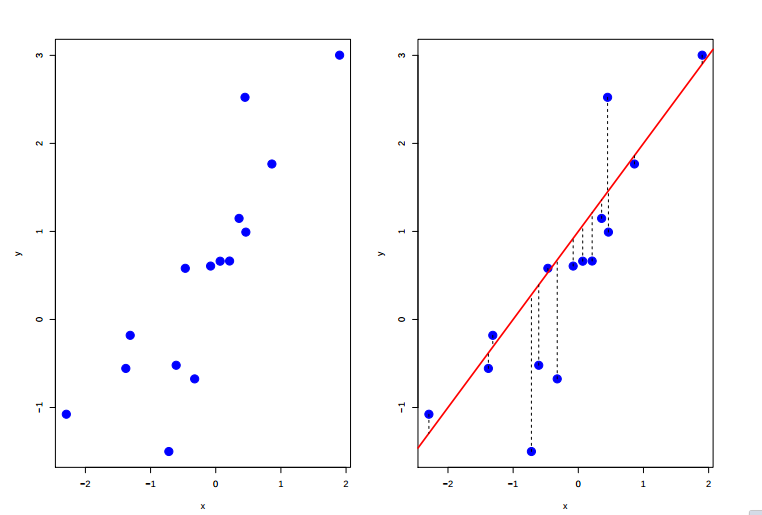
\includegraphics[scale = 0.6]{img/ejemploRectaRegresionLineal.png}
\end{center}
\end{example}

\paragraph{Cómo calcular la pendiente} de la recta de mínimos cuadrados.


Vamos a ver unas pocas maneras de calcular la recta de mínimos cuadrados.

\begin{itemize}

	\item El sistema habitual:

	\[ \hat{β}_1 = \frac{\sum_{i=1}^n(x_i - \bar{x})(Y_i - \bar{Y})}{\sum_{i=1}^n (x_i - \bar{x})^2} = \frac{S_{xy}}{S_{xx}} \]
	Donde
		\[S_{xy} = \sum_{i=1}^n(x_i - \bar{x})(Y_i - \bar{Y}) \]
		\label{Ssubxx}
		Y, consecuentemente, como el avispado lector podrá imaginar
		\[S_{xx} = \sum_{i=1}^n (x_i - \bar{x})^2\]

		Es interesante darse cuenta que, siendo $S_x$ la cuasivarianza, tenemos $S_{xx} = (n-1)S_x$


	\subitem \[β_0 = \bar{Y} - \hat{β}_1\bar{x}\]

	\textbf{Entonces:}
	\[\text{recta} \equiv y - \bar{y} = \frac{S_{xy}}{S_{xx}}(x - \bar{x} ) \]

	\item Mínimos cuadrados como promedio de pendientes:
	\label{rmc::promediopendientes}
	\[
	\hat{β}_1 = \frac{S_{xy}}{S_{xx}} = \sum_{i=1}^n \frac{(x_i - \bar{x})^2}{S_{xx}} \left( \frac{(Y_i - \bar{Y})}{x_i - \bar{x}} \right) = \sum_{i=1}^n ω_i \left( \frac{(Y_i - \bar{Y})}{x_i - \bar{x}} \right)
	\]

	Vemos que hemos ponderado la pendiente de cada recta que une cada punto con la media. Este peso es mayor cuanto mayor es la distancia \textbf{horizontal}.

	\item Mínimos cuadrados como promedio de respuestas:

	\[
	\hat{β}_1 = \frac{\sum_{i=1}^n  (x_i - \bar{x}) (Y_i - \bar{Y})}{S_{xx}} \overset{(1)}{=} \sum_{i=1}^n \frac{x_i-\gor{x}}{S_{xx}} Y_i = \sum α_i Y_i
	\]

	$(1) \impliedby$ hemos utilizado una propiedad básica, importantísima y, a simple vista, poco (o nada) intuitiva:

	\begin{prop}
	Sea $\{x_i\},\{y_i\}$ datos de variables aleatorias.
	\[
		\sum (x_i - \gor{x}) (y_i -\gor{y}) = \sum(x_i -\gor{x})y_i = \sum (y_i - \gor{y})x_i
	\]

	\textbf{Importante:} sólo quitamos la media de una de las 2. No podemos hacer $\sum (x_i - \gor{x}) (y_i -\gor{y}) = \sum x_iy_i$, porque esto ya no es verdad.
	\end{prop}
	\begin{proof}
		\[\sum_{i=1}^n (x_i - \gor{x}) (y_i -\gor{y}) = \sum_{i=1}^n (x_i -\gor{x})y_i - \underbrace{\sum_{i=1}^n (x_i-\gor{x})\gor{y}}_{0}\]

		Vamos a ver por qué ese término es 0.
	\[\sum_{i=1}^n (x_i-\gor{x})\gor{y} \overset{(1)}{=} \left(\left(\sum_{i=1}^n x_i\right) - n\gor{x}\right)\frac{\sum y_i}{n}\]

	$(1)\to$ Estamos restando $n$ veces el  término $\gor{x}$ que no tiene índice del sumatorio, con lo que podemos sacarlo fuera.


	Aplicando la propiedad distributiva con el factor $\frac{1}{n}$, obtenemos:


	\[
		\left(\frac{\left(\sum x_i\right)}{n} - \frac{n\gor{x}}{n}\right)\sum_{i=1}^n y_i = (\gor{x} - \gor{x}) \sum y_i = 0
	\]

	\obs Pero... ¿y porqué $\sum(x_i -\gor{x})y_i ≠ 0$? ¿Cuál es el fallo de lo siguiente?

	\[
		\sum(x_i -\gor{x})y_i = \frac{\sum(x_i -\gor{x})y_i}{n}·n
	\]
	¿Y aplicamos el mismo razonamiento que antes?

	La respuesta es que, en este caso el factor $(x_i-\gor{x})$ está multiplicado por $y_i$ \textbf{dentro} del sumatorio, es decir:

	\[
	\sum_{i=1}^n (x_i - \gor{x}) (y_i -\gor{y}) = \sum_{i=1}^n \left[(x_i -\gor{x})y_i\right] - \sum_{i=1}^n \left[(x_i-\gor{x})\gor{y}\right] \]
	Y podemos sacar $\gor{y}$ del sumatorio, porque está multiplicando y no tiene índice del sumatorio.

	\[ \sum_{i=1}^n \left[(x_i -\gor{x})y_i\right] - \sum_{i=1}^n \left[(x_i-\gor{x})\right]\gor{y}
	\]
	\end{proof}

	\begin{prop}Propiedades de estos $α_i$

		\begin{enumerate}
			\item $\sum α_i = 0$
				\begin{proof}
					\[\sum α_i = \sum \frac{(x_i-\gor{x})}{S_{xx}} = 0 \impliedby \sum (x_i-\gor{x}) = 0\]
					\[\sum (x_i-\gor{x}) = \left(\sum x_i\right) - n\gor{x} = \left(\sum x_i\right) - n \frac{\sum x_i}{n} = 0\]
				\end{proof}
			\item $\sum α_ix_i = 1$
				\begin{proof}
					\[ \sum α_ix_i = \sum\frac{(x_i-\gor{x})x_i}{S_{xx}} = \frac{1}{S_{xx}}\sum (x_i-\gor{x})(x_i-\gor{x}) = \frac{S_{xx}}{S_{xx}} = 1\]
				\end{proof}
			\item $\sum α_i^2 = \frac{1}{S_{xx}}$
				\begin{proof}
					\[\sum α_i^2 = \sum \frac{(x_i-\gor{x})(x_i-\gor{x})}{S_{xx}^2} = \sum \frac{(x_i-\gor{x})x_i}{S_{xx}^2} = \sum \frac{α_i x_i}{S_{xx}} = \frac{1}{S_{xx}} \sum α_ix_i \]
					Utilizando el anterior, tenemos $\sum α_i^2= \frac{1}{S_{xx}}$
				\end{proof}

		\end{enumerate}

	\end{prop}


\begin{defn}[Residuo]
En una recta de mínimos cuadrados: Sea $y_i = β_1x_i - β_0$ y sea $\hat{y}_i = \hat{β}_1x_i - \hat{β}_0$, llamamos residuo a $$e_i = y_i - \hat{y}_i$$

Los residuos cumplen:

\[
\sum_{i=1}^n e_i = 0
\]

Esto es intuitivo, ya que los errores se compensan y además es una buena propiedad.
\end{defn}
\begin{proof}
	En la recta de mínimos cuadrados calculamos $\hat{β}_0,\hat{β}_1$ con la finalidad de minimizar $\sum (y_i - β_0 - β_1x_i)^2$. Si recordamos, derivando respecto de $β_0$ obteníamos:

	\[\frac{∂}{∂β_0}\sum_{i=1}^n (y_i -  β_0 - β_1x_i)^2 = -2 \sum_{i=1}^n y_i -  β_0 - β_1x_i\]

	Y definimos $\hat{β}_0,\hat{β}_1$ como los parámetros que igualaban dicha derivada a $0$ (minimizaban la suma de diferencias al cuadrado), es decir $\hat{β}_0,\hat{β}_1$ cumplen:

	\[\sum_{i=1}^n y_i -  \hat{β}_0 - \hat{β}_1x_i = 0\]

	Pero precisamente $\hat{y}_i=\hat{β}_0 + \hat{β}_1x_i$ y por tanto tenemos que:

	\[\sum_{i=1}^n y_i - \hat{y}_i = \sum_{i=1}^n e_i = 0\] 
\end{proof}



\begin{prop}
Sean $\{e_i\}$ una variable aleatoria que cumple \footnote{Se ha utilizado la $e$ porque es útil en cuanto a los residuos de la recta de mínimos cuadrados}:
\[\sum e_i = 0\]

Entonces:
\[\sum e_i x_i = 0 \implies \cov{e,x} = 0\]
\end{prop}

\begin{proof}
\[
\cov{e,x} = \esp{e}\esp{x} - \esp{e·x}
\]

Vamos a ver que los 2 sumandos son 0.

 $\esp{e}\esp{x} = 0 \impliedby \esp{e} \overset{?}{=} \gor{e} = 0$


Por otro lado:
\[ \sum (e_i - \vec{µ}) x_i = \sum (e_i - \vec{µ}) (x_i - \vx) \]


\[
\esp{e·x} = \sum e_ix_i = \sum e_ix_i - \vx \sum e_i = \sum e_i(x_i - \vx)
\]
\end{proof}


Esto tiene la siguiente explicación ``intuitiva'': La recta de mínimos cuadrados contiene toda la información lineal que $X$ puede dar sobre $Y$ (debido a que la covarianza entre los residuos y $X$ es 0).
\end{itemize}

\subsubsection{Fallos de la recta de mínimos cuadrados}

Vamos a ver un par de ejemplos ilustrativos:

\begin{example}[Sobre los datos atípicos]

Esta es una recta de mínimos cuadrados calculada para una nube de puntos a la que se ha añadido un punto atípico. Se ve una cierta tendencia de que la pendiente debería ser positiva, pero el dato atípico provoca un cambio brusco.
\begin{center}
%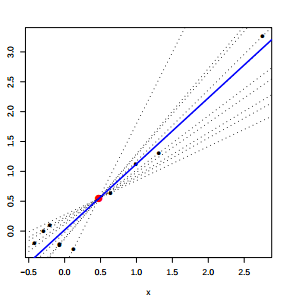
\includegraphics[scale=0.9]{img/rmc_atipico1.png}
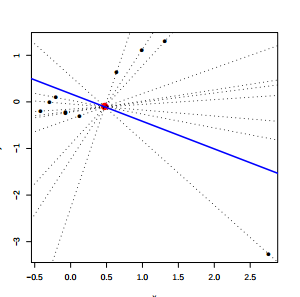
\includegraphics[scale=0.9]{img/rmc_atipico2.png}
\end{center}

\end{example}

\begin{example}[Sobre la distancia horizontal]
\label{ej:reg_simple}
¿Y da igual lo atípico que sea un dato? La respuesta es que no. Si el dato es muy atípico en la variable respuesta ($Y$), pero es muy \textit{típico} en la variable regresora, la recta no se desvía tanto. Vamos a verlo y después explicamos la razón.

Esta es la recta, en la que hemos ignorado los 3 datos que parecen ``atípicos''.
\begin{center}
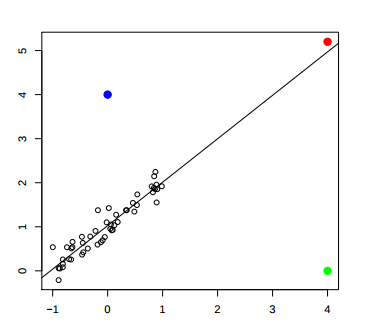
\includegraphics[scale=0.9]{img/sobredistanciahorizontal.png}
\end{center}

Ahora calculamos las rectas teniendo en cuenta sólo uno de los puntos.

\begin{center}
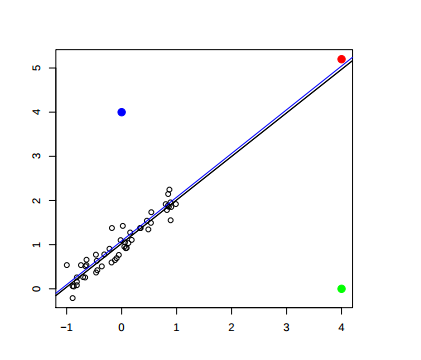
\includegraphics[scale=0.4]{img/sobredistanciahorizontal1.png}
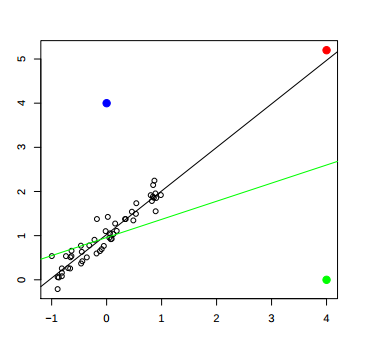
\includegraphics[scale=0.4]{img/sobredistanciahorizontal2.png}
\end{center}

Vemos que la recta azul no se desvía apenas de la original, mientras que la recta verde si se desvía un montón. ¿Esto a qué se debe? A que importa más la distancia horizontal de la media que la distancia vertical. Si vamos a la expresión de la recta de mínimos cuadrados como promedio de las pendientes \ref{rmc::promediopendientes} vemos que hay un término $\frac{(x_i - \gor{x})}{S_{xx}}$ que hemos tomado como pesos para ponderar y en este caso, la distancia horizontal $(x_i - \gor{x})$ está multiplicando en el numerador.



\end{example}





\subsubsection{Introduciendo ``aleatoreidad'' para poder hacer IC}

Sea $\{ε_i\}$ siendo $ε_i \sim N(0,σ^2)$. Lo habitual es no saber cómo han sido generados los datos y es probable que no vayamos a conocer con exactitud absoluta la recta de mínimos cuadrados. Es por ello que suponemos el siguiente modelo para la variable respuesta:

\[
Y_i = β_1 x_i + β_0 + ε_i
\]


Tenemos que $\bar{y}_i \sim N$, ya que es una combinación lineal de variables normales \textbf{independientes} (como vimos en el Tema 1).


\begin{example}
Sea $σ=1, β_0 = 0$ y $β_1 = 1$.

Entonces el modelo es:

\[
Y_i = x_i + ε_i
\]

Fijamos $n=10$ y generamos las respuestas para $x_i = i$. Además, repetimos el experimento 6 veces y calculamos las rectas de mínimos cuadrados, obteniendo:

\begin{center}
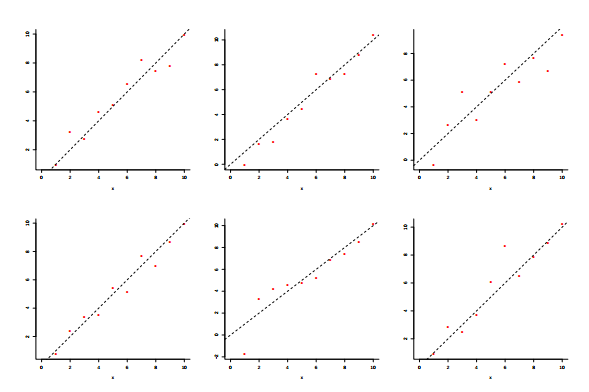
\includegraphics[scale=0.6]{img/6ejemplosRegresion.png}
\end{center}

Vemos que obviamente las rectas no son las mismas. Esto se debe al $ε_i$ introducido. ¿Cuáles son los valores que toman $β_1$ y $β_0$? Habiendo repetido el experimento 1000 veces, obtenemos los siguientes histogramas:

\begin{center}
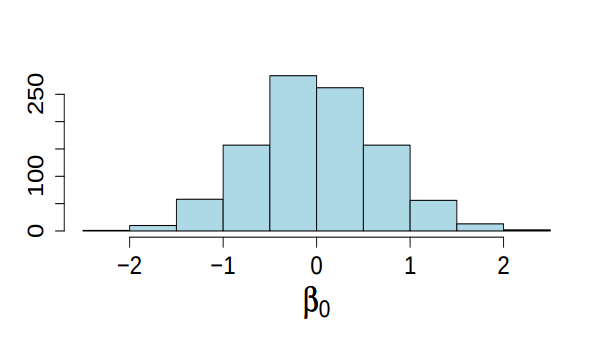
\includegraphics[scale=0.3]{img/1000vecesb0.png}
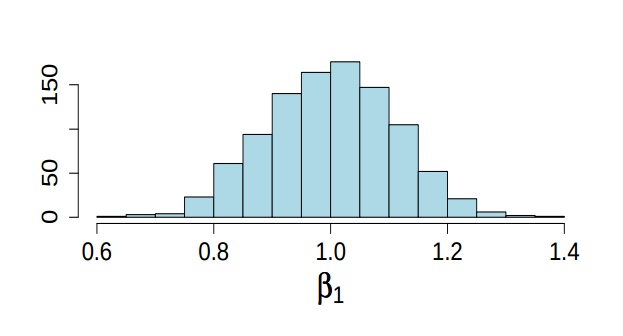
\includegraphics[scale=0.3]{img/1000vecesb1.png}
\end{center}

Vemos que no siempre es el mismo valor. Sabemos (por cómo hemos construido los datos) que $β_0 = 0$ y $β_1 = 1$, pero nuestra manera de calcularos (debido a $ε_i$) no siempre nos da el valor concreto.


\end{example}

El ejemplo anterior nos muestra que en realidad, estamos estimando $β_i$, aunque no nos guste y ahora tenemos que plantearnos ¿Cómo de buenos son nuestros estimadores? Tal vez son una mierda, o tal vez son insesgados.

Para ello, vemos que al haber añadido un error $\epsilon_i \sim N(0,σ^2)$, tenemos:

\[
Y_i = β_0 + β_1x + ε_i \implies Y_i \equiv N(β_0 + β_1X_i, σ^2)
\]


\subsubsection{Estimando $β_1$}

\begin{prop}
Nuestro estimador ``pendiente de la recta de mínimos cuadrados:'' $\hat{β}_1$  cumple

\[
\hat{β}_1 \equiv N\left(β_1,\frac{σ^2}{S_{xx}} \right)
\]

\end{prop}

\begin{proof}

\begin{itemize}
	\item $\esp{\hat{β}_1} = \sum_{i=1}^nα_i \mathbb{E}(Y_i) = \sum_{i=1}^n α_i(β_0+β_1x_i) = β_0 \underbrace{\sumα_i}_{=0} + β_1 \underbrace{\sum α_ix_i}_{=1} = β_1$
	\item $\var{\hat{β}_1} = \mathbb{E}(\hat{β}_1^2) - \mathbb{E}^2(\hat{β}_1) = \var{\sum_{i=1}^nα_iy_i} \underbrace{=}_{y_i\text{ independientes}} \sumα_i^2σ_i^2 \underbrace{=}_{\text{homocedasticidad}} \displaystyle\frac{σ^2}{S_{xx}}$
\end{itemize}
\end{proof}

\subsubsection{Estimando $β_0$}

\begin{prop}
Nuestro estimador ``término independiente de la recta de mínimos cuadrados:'' $\hat{β}_0$  cumple

\[
\hat{β}_0 = N\left(β_0 , σ^2 \left( \frac{1}{n} + \frac{\gor{x}^2}{S_{xx}}\right)  \right)
\]
\end{prop}

\begin{proof}
\begin{itemize}
	\item $\esp{\hat{β}_0} = β_0$
	\item
	$\var{\hat{β}_0} = \var{\gor{Y}} + \var{\hat{β}_1\gor{x}} - 2· \cov{\gor{Y},\hat{β}_1\gor{x}} = \frac{σ^2}{n} + \gor{x}^2\frac{σ^2}{S_{xx}} - 2\gor{x}·\cov{\gor{Y}, \hat{β}_1}$

 	\subitem Calculamos: $\cov{\gor{Y},\hat{β}_1}$ utilizando cosas del tema 1

 	\[
		\cov{\gor{Y},\hat{β}_1} = \cov{\frac{1'_n Y}{n},α'Y} = \frac{1}{n}1'_nσ^2Iα = 0
 	\]
 	debido a que $α = 0$.

 	Ademas de ser incorrelados, son \textbf{independientes}. ¿Por qué? Porque conjuntamente son normales, es decir \[
 		\begin{pmatrix} \gor{Y} \\ \hat{β}_1 \end{pmatrix} \equiv A\gor{Y} \equiv N_2
 	\]
\end{itemize}

\end{proof}


\textbf{Conclusiones:}
\begin{align*}
\gor{Y} &\text{ es independiente de } \hat{β}_1\\
\hat{β}_1 &\equiv \left(β_1,\frac{σ^2}{S_{xx}}\right)\\
\hat{β}_0 &\equiv \left(β_0,σ^2 \left( \frac{1}{n} + \frac{\gor{x}^2}{S_{xx}}\right)\right)
\end{align*}

¿Son estas las variables $\hat{β}_1 $ y $\hat{β}_0$ normales una normal conjunta? Sí, \textbf{sí son una normal conjunta}. Una manera que tenemos de saber si es una normal conjunta es si son independientes, y en este caso no lo son.  Intuitivamente es fácil de ver. En una recta, si aumentamos la pendiente (y estamos en el primer cuadrante) entonces el término independiente disminuye.

Esta dependencia tiene que aparecer. Vamos a estudiar la covarianza entre los estimadores:

\[
\cov{\hat{β}_0,\hat{β}_1} = \cov{\gor{Y} - \hat{β}_1\gor{x}, \hat{β}_1} = \cov{\gor{Y}, \hat{β}_1} - \gor{x}\cov{\hat{β}_1, \hat{β}_1} = -\gor{x}\frac{σ^2}{S_{xx}}
\]


Pero sabemos que sí son una normal bidimensional porque toda combinación lineal de nuestros parámetros de la recta es una variable aleatoria (la variable regresora $\hat{Y}$) normal. Es decir:
\[\left(\begin{array}{c} \hat{β}_0\\ \hat{β}_1\end{array}\right) = AY\]


\subsubsection{IC y Contrastes para $β_1$}
\label{subsubsec:ICparaB1}

Recordamos que \[ \hat{β}_1 \equiv N\left(β_1,\frac{σ^2}{S_{xx}}\right)\]

Podemos normalizar y buscar una cantidad pivotal (como hacíamos en estadística I)

\[
\frac{\hat{β}_1 - β_1}{\frac{σ}{\sqrt{S_{xx}}}} \equiv N\left(0,1\right)
\]

Pero aquí nos encontramos con que necesitamos $σ$, la varianza de los errores. Esta varianza a menudo no es conocida (porque no sabemos con exactitud cuál es la recta verdadera) y tenemos que estimarla.

Para estimarla, parece razonable usar \[ \hat{σ} = S_R =\frac{\sum_{i=1}^n e_i^2}{n-2}\]

\begin{expla}
Recordamos que para que estimar la varianza, utilizamos (por el lema de Fisher) $n-1$ de denominador para que el estimador sea insesgado. Esto sale de que en la demostración, hay una matriz de rango $n-1$ ya que existe una restricción.

Siguiendo este razonamiento, en este caso tenemos 2 restricciones\footnote{$\sum e_i = 0$ y $\sum e_ix_i = 0$}, por lo que si lo demostráramos rigurosamente, aparecería una matriz de rango $n-2$ y por eso es el denominador. De esta manera, conseguimos un estimador insesgado.

\end{expla}

Además, $S_R$ se denomina \concept{Varianza\IS residual}

\begin{prop}
Una pequeña generalización del lema de Fisher:
\[
\frac{(n-2)S_{R}^2}{σ^2} \equiv \chi_{n-2}^2
\]

Además, es independiente de $\hat{β}_1$

\end{prop}



\begin{proof}
Esta proposición es un caso particular de un teorema que veremos más adelante.
\end{proof}


Llamamos
\[ P_{R} = \frac{\hat{β}_1-β_1}{\frac{S_R}{\sqrt{S_{xx}}}}\]
\[ P_σ = \frac{\hat{β}_1-β_1}{\frac{σ}{\sqrt{S_{xx}}}}\]

Sabemos que $P_σ \sim N(0,1)$. Pero, al estimar ¿Se mantiene$P_R \sim N(0,1)$?

Al estimar $σ$,  $P_{R}$ no tiene porqué ser exactamente $N(0,1)$. Si $n\to ∞$, entonces $S_R = σ$ y entonces $P_σ = P_R = N(0,1)$, pero para otros valores de $n≠∞$...

Por ello, nos vemos en la necesidad de manipular $P_R$ algebraicamente a ver si conocemos qué distribución tiene (que debería ser algo cercano a una normal, ya que estamos estimando $σ$ con un estimador insesgado. Tal vez las colas de la distribución son menos pesadas y podríamos esperar que fuera una $t$)

\label{Cuentas:largas}

\[
\displaystyle\frac{\hat{β}_1-β_1}{\displaystyle\frac{S_R}{\sqrt{S_{xx}}}} = \displaystyle\frac{\hat{β}_1-β_1}{\displaystyle\frac{σ}{\sqrt{S_{xx}}}\frac{S_R}{σ}} = \left( \displaystyle\frac{\hat{β}_1-β_1}{\displaystyle\frac{σ}{\sqrt{S_{xx}}}} \right)\displaystyle\frac{1}{\displaystyle\frac{S_R}{σ}} = \displaystyle\frac{ \displaystyle\frac{\hat{β}_1-β_1}{\frac{σ}{\sqrt{S_{xx}}}} }{\displaystyle\frac{S_R}{σ}}
\]

En el numerador tenemos una $N(0,1)$ y en el denominador la raíz de una $\chi^2$ dividida por sus grados de libertad (por la proposición anterior). Esto es por definición una $t$ (T-Student) con los mismos grados de libertad que la $\chi^2$, es decir $n-2$. (\href{https://en.wikipedia.org/wiki/Student%27s\_t-distribution#Characterization}{Wikipedia})


\begin{prop}
Podemos calcular el intervalo de confianza  para la pendiente de la recta, utilizando la fórmula de intervalo de confianza

\[
IC_{1-α}(β_1) \equiv \left[ \hat{β}_1 \mp t_{n-2,\frac{α}{2}}\frac{S_R}{\sqrt{S_{xx}}}\right] = \left[ \hat{β}_1 \mp \mathcal{Z}\frac{σ}{\sqrt{S_{xx}}}\right] %\equiv \left[ \gor{Y} \mp \t_{n-1,\frac{α}{2}}\frac{S_R}{\sqrt{n}} \right]
\]
\end{prop}

\subsubsection{Contraste en R}

\label{example:R-output}
\begin{lstlisting}[style=mystyle]
# Ajusta el modelo
regresion = lm(Fracaso~Renta)
summary(regresion)

lm(formula = Fracaso ~ Renta)

Residuals:	Min		1Q			Median		3Q		Max
				-7.8717 -3.7421		0.5878	3.0368	11.5423
---
Coefficients:	Estimate Std.	Error 	t-value		Pr(>|t|)
(Intercept)		38.4944				3.6445	10.562		8.37e-10 ***
Renta 				-1.3467				0.2659	-5.065		5.14e-05 ***
---
Signif. codes: [...]
Residual standard error: 4.757 on 21 degrees of freedom
Multiple R-Squared: 0.5499,
Adjusted R-squared: 0.528
\end{lstlisting}


Aquí, la fila de \textit{intercept} es el término independiente y renta es la pendiente. Además, los p-valores son para el contraste $\hat{β_i} = 0$, dentro de la hipótesis $β_i \geq 0$. \footnote{Si queremos contrastar si es positivo, nos vamos al caso límite que lo separa y contrastamos eso}.

En este caso, el p-valor para $H_0: \hat{β}_1=$ es $5.14e-5$, con lo que no podemos rechazar la hipótesis.


\subsubsection{Predicciones}

Sea $(x_1,y_1),...,(x_n,y_n) \to y_i = β_0 + β_1x_i + ε_i$.

Dado una nueva observación $x_0$, tenemos 2 problemas para predecir:

\begin{itemize}
	\item \textbf{Inferencia sobre $m_0 \equiv \esp{y_0 | x_0} = β_0 + β_1x_0$}

	En este caso, $$\hat{m}_0 = \hat{β}_0 + \hat{β}_1x_0$$

	¿Cómo es este estimador?

	\[\esp{\hat{m}_0} = β_0 + β_1x_0 = m_0\]
	\[\var{\hat{m}_0} = ... = σ^2\left[\frac{1}{n} + \frac{(x_0-\bar{x})^2}{S_{xx}} \right] \]

	\subitem Intuitivamente, lo que significa el segundo sumando de la varianza es que ``cuanto más cerca esté $x_0$ de la media, mejor será la estimación''.

	\textbf{Conclusión:}

	\[
		\hat{m}_0 \sim N\left( m_0, σ^2\left[\frac{1}{n} + \frac{(x_0-\bar{x})^2}{S_{xx}} \right]\right)
	\]



	\subitem \textbf{Intervalo de confianza} para $m_0$ utilizando la fórmula de intervalos de confianza:

	\[
IC_{1-α}(m_0) \equiv \left[ \hat{m}_0 \pm t_{n-2,\frac{α}{2}}S_R\sqrt{\frac{1}{n} + \frac{(x_0 - \gor{x})^2}{S_{xx}}}\right]
\]

	\item \textbf{Predecir $Y_0$} usamos de nuevo:

	\[
\hat{Y}_0 = \hat{β}_0 + \hat{β}_1x \to Y_0 - Y \equiv N\left( 0, σ^2\left( 1 + \frac{1}{n}+  \frac{(x_0-\gor{x})^2}{S_{xx}}\right) \right)
	\]

	Donde la varianza ha sido calculada:

	\[
	\var{Y_0 - \hat{Y}_0} = \underbrace{\var{Y_0}}_{σ^2} - \underbrace{\var{\hat{Y}_0}}_{σ^2(\frac{1}{n}+\frac{(x_0-\gor{x})^2}{S_{xx}})} + \underbrace{2 \cov{Y_0,\hat{Y}_0}}_{ = 0 \text{ (indep.) }} = σ^2 + σ^2\left( \frac{1}{n}+  \frac{(x_0-\gor{x})^2}{S_{xx}} \right)
	\]


	Este es un problema más complicado, ya que tenemos que tener en cuenta el término de error $ε_i$ y es por esto que aparece el 1 en la varianza. Tenemos que tener en cuenta la incertidumbre.

	Estandarizando y cambiando $σ$ por $S$, tenemos:

	\[
	\frac{Y_0 - \hat{Y}_0}{S_R \sqrt{1 + \frac{1}{n} + \frac{(x_0-\gor{x})^2}{S_{xx}}}} \equiv t_{n-2}
	\]

	Ya que tenemos una normal estandarizada dividida por su .... que por definición, es una $t$ de student.

	Ahora, vamos a construir el \concept{intervalo de predicción} (cambia ligeramente la interpretación)

	\[
1 - α = P\left\{ -t_{n-2;\frac{α}{2}} < \frac{Y_0 - \hat{Y}_0}{ET(Y_0-\hat{Y}_0)} < t_{n-2;\frac{α}{2}}    \right\} = P \left\{ Y_0 \in \left[ \hat{Y}_0 \pm t_{n-2;\frac{α}{2}} S_R \sqrt{1+\frac{1}{n}+\frac{(x_0-\gor{x})^2}{S_{xx}}} \right]  \right\}
	\]
\end{itemize}

Ahora vamos a hacer unos ejemplos numéricos.

\begin{example}Seguimos con el ejemplo de la renta.
\begin{problem}
\begin{center}
\begin{tabular}{c|c|c}
&media&desviación típica\\\hline
\% fracaso & 20.73 & 6.927\\
renta &13.19  & 3.814
\end{tabular}
La renta está expresada en miles de euros.
\end{center}


\ppart IC para $β_1$ de nivel $95\%$.
\ppart IC para \% de fracaso medio si la renta es de $14.000$ euros.


Es parte del enunciado la salida de ``R'' incluida en: \ref{example:R-output}

\solution
\spart

\[
IC_{1-α}(β_1) = \left[-1.3467 \mp t_{21;0.025} · (0.2659)\right]
\]

Donde el $-1.3467$ es el estimador $\gor{β_1}$ que obtenemos de la salida de $R$. Lo mismo el $0.2659$, que es el error típico.

\spart
\[ \gor{Y_0} = 38.49 - (1.3467) · \underbrace{14}_{x_0} = 19.64\]

Siendo este el estimador, vamos a construir el intervalo de confianza. \footnote{Podría ser que nos pidieran el intervalo de predicción, pero en ese caso estarían pidiendo el intervalo de ...... para predecir. Además, nos están dando un $x_0$ que para predicción no lo tenemos}

\[
IC_{1-α}(m_0) = \left[19.64 \mp (2.06)(4.757)\sqrt{\frac{1}{23}+\frac{(14-13.19)^2}{S_{xx}}}\right]
\]
Donde $S_{xx} = 320.06$ y podemos calcularlo despejando de:

\[
E.T.(\gor{β_1}) = \sqrt{\frac{S_R^2}{S_{xx}}} \to \sqrt{S_{xx}} = \frac{4.757}{0.2659} \to S_{xx} = 320.06
\]
Donde $E.T.(\gor{β_1})$ es el error típico dado por \textit{R}. En este caso es $0.2659$y $S_R^2 = 4.757^2$

También podríamos utililzar $S_x = \frac{S_{xx}}{n-1}$, sabiendo que $S_x^2 = \frac{n}{n-1}σ^2$. Sabemos que $S_x = 3.814$ por ser la renta la variable explicativa, es decir, las $x$ de nuestro modelo de regresión.

\[
\frac{n}{n-1}\left(3.814\right)^2 = \frac{S_{xx}}{n-1} \to S_{xx} = 21·\left(3.814^2·\frac{22}{21}\right) = 320.03
\]
\end{problem}


\end{example}


\obs Todos estos cálculos y todas estas fórmulas se basan en muchas hipótesis (como que la distribución del error sigue una distribución normal). Pero podría ser que esto no ocurriera y estuviéramos suponiendo un modelo falso. Para ello, en estadística existe el \concept{Diagnóstico del modelo}. Este diagnóstico, consiste en comprobar si las hipótesis del modelo son \textbf{aceptables} para los datos disponibles. ¡Ojo! Aceptable... Puede haber muchos modelos aceptables para un mismo conjunto de datos.

Este diagnóstico se suele basar en el análisis de los residuos del modelo.

\begin{example}
	Vamos a ver a ojo unos cuantos ejemplos. Vamos a utilizar que $\corr{e,\gor{y}} = 0$ bajo el modelo (como calculamos anteriormente)

\begin{center}
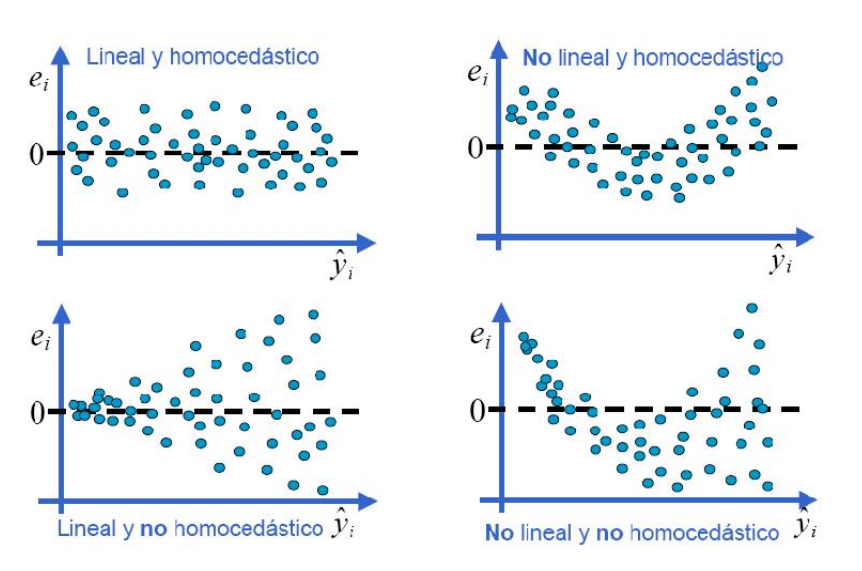
\includegraphics[scale=0.5]{img/diagmodelo.png}
\end{center}

De estos 4 gráficos, el bueno es el primero, ya que los demás no cumplen alguno.
\end{example}

\begin{example}
Vamos a ver otro ejemplo, donde arriba están los datos y abajo los residuos. Mirando sólo la fila de arriba podríamos saber si nuestro modelo para la regresión se cumple o sino.


\begin{center}
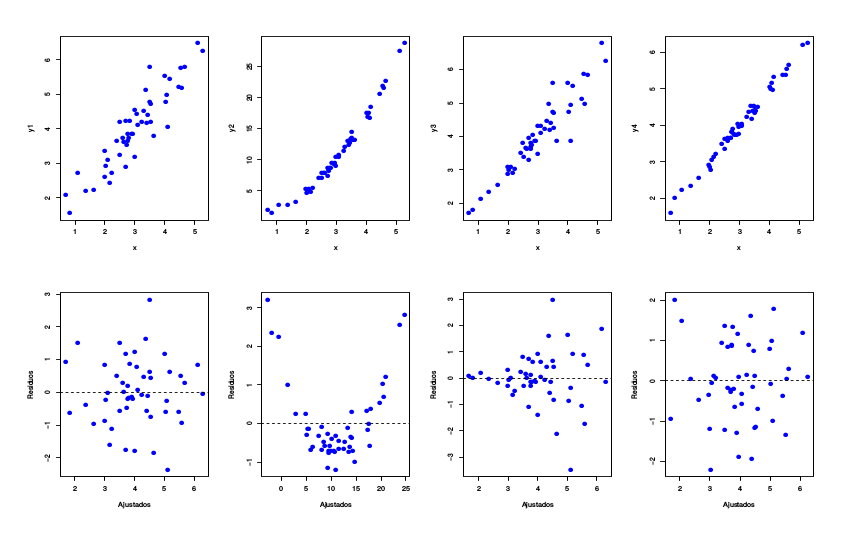
\includegraphics[scale=0.5]{img/diagmodelo_2.png}
\end{center}

Vemos que el primero y el último si tienen este modelo como aceptable, ya que en los residuos no hay ningún patrón (y se cumple que la correlación es 0).

En el segundo, podríamos suponer que es bueno, pero al diagnosticar el modelo mirando los residuos, vemos que no. El diagnóstico del modelo \textbf{magnifica los errores}.

En el cuarto, vemos más claro que es heterocedástico y que no se cumple el modelo supuesto.
\end{example}

En regresión múltiple veremos que no podemos ver los datos, ya que son demasiadas variables, pero sí podemos estudiar los residuos como acabamos de hacer en los ejemplos anteriores.


\subsection{Regresión lineal múltiple}

\label{example:fuel2001}
El ejemplo que vamos a estudiar en regresión múltiple es el consumo de gasolina en EEUU intentando predecirlo a partir de unas cuantas variables. Las variables regresoras son:

\begin{center}
\begin{tabular}{cccccccc}
State&Drivers&FuelC&Income&Miles&MPC&Pop&Tax\\\hline
AL&3559897&2382507&23471&94440&12737.00&3451586&18.0\\
AK&472211&235400&30064&13628&7639.16&457728&8.0\\
AZ&3550367&2428430&25578&55245&9411.55&3907526&18.0
\end{tabular}
\end{center}


Estos son los datos que obtenemos de $R$:

\begin{lstlisting}[style=mystyle]
reg <- lm(FuelC ~ Drivers+Income+Miles+MPC+Tax, data=fuel2001)
summary(reg)

Coefficients:
              Estimate Std. Error t value Pr(>|t|)
(Intercept) -4.844e+05  8.102e+05  -0.598 0.552903
Drivers      6.144e-01  2.229e-02  27.560  < 2e-16 ***
Income       7.526e+00  1.611e+01   0.467 0.642587
Miles        5.813e+00  1.587e+00   3.664 0.000652 ***
MPC          4.643e+01  3.488e+01   1.331 0.189820
Tax         -2.114e+04  1.298e+04  -1.629 0.110298
---
Signif. codes:  0 '***' 0.001 '**' 0.01 '*' 0.05 '.' 0.1 ' ' 1

Residual standard error: 394100 on 45 degrees of freedom
Multiple R-squared:  0.9808,	Adjusted R-squared:  0.9787
F-statistic: 459.5 on 5 and 45 DF,  p-value: < 2.2e-16

\end{lstlisting}

\subsubsection{Notación}


\begin{itemize}
	\item $n$ es el número de observaciones, en este caso, el número de estados.
	\item $k$ es el número de atributos.
	\item $ε_i \sim N(0,σ^2)$
	\item $n\geq k+2$: esta hípótesis  es muy necesaria.\footnote{En la estadística, habría que rehacer el modelo para cuando $k>n$. ¿Y cuándo $k>n$? ¿Cuándo puede ocurrir esto? Cada vez más hay más información para cada individuo. En estudios genéticos por ejemplo, que hay millones de genes pero no se pueden hacer el estudio con millones de personas... \textbf{LA MALDICIÓN DE LA DIMENSIONALIDAD} que decimos en Introducción previa a los Fundamentos Básicos del Aprendizaje Automático.\\ Una posible solución al problema es un algoritmo que filtre los atributos que son importantes.}
\end{itemize}

Regresión simple es un caso particular de múltiple, tomando $k=1$.

\subsubsection{Modelo}

Tenemos una muestra de $n$ observaciones de las variables $Y$ y $X_1,…,X_k$. Para la observación $i$, tenemos el vector $(Y_i,x_{i1},x_{i2},…,x_{ik})$.

El modelo de regresión lineal múltiple supone que:
\[Y_i=β_0+β_1x_{i1}+…+β_kx_{ik}+ε_i,\ i=1,...,n\]

donde las variables de error $ε_i$ verifican:
\begin{enumerate}
\item $ε_i$ tiene media cero, para todo $i$.
\item Var($ε_i$) = $σ^2$, para todo $i$ (homocedasticidad).
\item Son variables independientes.
\item Tienen distribución normal.
\item $n ≥ k + 2$ (hay más observaciones que parámetros).
\item Las variables $X_i$ son linealmente independientes entre sí (no hay colinealidad).
\end{enumerate}

Las 4 primeras hipótesis se pueden reexpresar así: las observaciones de la muestra son independientes entre sí con
\[Y_i \equiv N(β_0 +β_1x_{i1} +...+β_kx_{ik},σ),\ i=1,...,n\]

En forma matricial:

\[
	\begin{pmatrix}
		Y_1\\
		Y_2\\
		\vdots \\
		Y_n
	\end{pmatrix}
	=
	\begin{pmatrix}
		1 & x_{11} & … & x_{1k} \\
		1 & x_{21} & … & x_{2k} \\
		\vdots & \vdots &  & \vdots \\
		1 & x_{n1} & … & x_{nk}
	\end{pmatrix}
	\begin{pmatrix}
		β_1\\
		β_2\\
		\vdots \\
		β_n
	\end{pmatrix}
	+
	\begin{pmatrix}
		ε_1\\
		ε_2\\
		\vdots \\
		ε_n
	\end{pmatrix}
\]


De forma más compacta, el modelo equivale a:
\[Y =Xβ+ε,\ ε \equiv N_n(0,σ^2I_n) \iff Y \equiv N_n(Xβ,σ^2I_n)\]

\begin{defn}[Matriz de diseño]
	La matriz $X$ se conoce como matriz de diseño
\end{defn}

\subsubsection{Estimación de los parámetros del modelo}

La pregunta que lógicamente se nos viene a la cabeza en este momento es: ¿Cómo estimar $β$ a partir de $Y$ y $X$?. Para ello nos serviremos de la interpretación geométrica del modelo:

Sea $\mathcal{V} ⊂ R^n$ el subespacio vectorial generado por las columnas de la matriz de diseño $X$ ($\dim(\mathcal{V}) = k + 1$).
\[μ∈\mathcal{V} \iff ∃β∈R^{k+1} : μ=Xβ\]
El modelo equivale a suponer $Y \equiv N_n(μ, σ^2I_n)$, donde $μ ∈ \mathcal{V}$.

\newpage
\begin{figure}[hbtp]
	\centering
	\inputtikz{proyecta_V}
\end{figure}

Con esto, parece razonable estimar $µ$ mediante la proyección ortogonal de $Y$ sobre $\mathcal{V}$ para obtener $\hat{Y} = X\hat{β}$. Equivalentemente: $\norm{Y-X\hat{β}}^2 \leq \norm{Y-Xβ}^2, ∀β\in ℝ^{k+1}$

\begin{defn}[Estimador mínimos cuadrados]

	Al $\hat{β}$ que minimiza
	\[\norm{Y - Xβ}^2 = \sum_{i=1}^n (Y_i - β_0 - β_1x_{i1} - … - β_kx_{ik})^2\]
	se le denomina estimador de mínimos cuadrados.
\end{defn}

Veamos qué podemos sacar de lo visto hasta ahora para averiguar quién es exactamente $\hat{β}$:

Para que $\hat{Y}$ sea la proyección de $Y$ sobre $\mathcal{V}$ es necesario y suficiente que se satisfagan las ecuaciones normales:

\begin{defn}[Ecuaciones normales]
	Tomando $e = Y - \hat{Y}$ como el vector residuo, las ecuaciones normales se satisfacen si:
	\[X'(Y - \hat{Y})=0 \iff X'e = 0\]
\end{defn}

Que se satisfagan estas ecuaciones es equivalente a decir que la resta $Y - \hat{Y}$ da un vector perpendicular a la base $\mathcal{V}$. Sustituyendo $\hat{Y} = X\hat{β}$:

\[X'(Y - X\hat{β}) = 0 \iff X'Y = X'X\hat{β}\]

Ya que las filas de $X'$ (las columnas de $X$) son independientes, sabemos que $X'X$ tiene rango completo y por tanto es invertible. Y llegamos a la expresión para nuestro estimador de mínimos cuadrados $\hat{β}$:
\begin{equation}
	\boxed{\hat{β} = (X'X)^{-1}X'Y}
\end{equation}


\begin{obs}
	En regresión simple se tiene que:
	\[
		X\equiv
		\begin{pmatrix}
			1 & x_1\\
			\vdots & \vdots \\
			1 & x_n
		\end{pmatrix}
		\text{ y que: }
		X'X =
		\begin{pmatrix}
			n & \sum x_i \\
			\sum x_i & \sum x_i^2
		\end{pmatrix}
	\]
\end{obs}

Con lo visto hasta el momento sabemos que $\hat{Y} = X\hat{β} = X(X'X)^{-1}X'Y$, es decir, que nuestra $\hat{Y}$ está expresada como producto de $Y$ por una matriz que llamaremos:

\begin{defn}[Hat matrix]
	\[H = X(X'X)^{-1}X'\]
	se conoce como hat matrix, puesto que da $Y$ gorro: $\hat{Y} = HY$.
\end{defn}

La hat matrix $H$ tiene las siguientes \textbf{propiedades}:
\begin{itemize}
	\item Es matriz de proyección ortogonal sobre $\mathcal{V}$.
	\item Es simétrica e idempotente.
	\item Tiene rango $k+1$ (la dimensión del espacio $\mathcal{V}$ sobre el que proyecta).
\end{itemize}

\begin{obs}
	Podemos servirnos de la hat matrix para expresar el vector de residuos:
	\[e = Y - \hat{Y} = Y - HY = (I - H)Y\]
	Donde $(I-H)$ es una matriz simétrica e idempotente con rango $rg(I-H)=~n-~(k~+~1)$, que proyecta sobre el espacio ortogonal $\mathcal{V}^\perp$.
\end{obs}

Para acabar esta sección enumeramos algunas propiedades de los parámetros:
\begin{itemize}
\item $\hat{β}$ es el estimador de máxima verosimilitud (EMV) de $β$:
\[L(β,σ)= \left(\frac{1}{\sqrt{2π}σ}\right)^n exp\left\{-\frac{1}{2σ^2} \norm{Y−Xβ}^2 \right\}.\]

\item El EMV de $σ^2$ es:
\[\hat{σ}^2 = \frac{\norm{Y−Xβ}^2}{n} = \frac{\norm{e}^2}{n} = \frac{\sum_{i=1}^n e_i^2}{n}\]

\item El vector $\hat{β}$ tiene distribución $N_{k+1}(β, σ^2(X′X)^{−1})$ (en la siguiente sección se demuestra).
\end{itemize}

\subsubsection{Estudio de la varianza residual}
Un estimador insesgado de $σ^2$ es la varianza residual $S_R^2$ , es decir, la suma de los residuos al cuadrado, corregida por los grados de libertad apropiados (en este caso $n-\dim{(\mathcal{V})}$):
\[S_R^2 = \frac{\sum e_i^2}{n-(k+1)} = \frac{\norm{e}^2}{n-k-1} = \frac{\norm{Y - \hat{Y}}^2}{n-k-1}\]

Si nos fijamos en que:
\[\norm{Y - \hat{Y}}^2 = Y'(I-H)(I-H)Y = Y'(I-H)Y\]

y sabiendo que la matriz $I-H$ es simétrica e idempotente, si recordamos la proposición \ref{prop:tema1_pepino} y demostramos $μ(I-H)μ'=0$, podemos determinar que la distribución de $S_R^2$:

Dado que $μ∈\mathcal{V}$ y sabiendo que $μ=XB$:
\[(I-H)μ = (I-H)XB = 0\]
Ya que el vector $(I-H)$ proyecta sobre $\mathcal{V}^\perp$.

Así llegamos a que:
\[\frac{\norm{Y-\hat{Y}}^2}{σ^2} = \frac{Y'(I-H)Y}{σ^2}=\]
\begin{equation}
	\boxed{\frac{(n-k-1)S_R^2}{σ^2} \equiv χ_{n-k-1}^2}
\end{equation}


Además si tomamos esperanzas en ambos lados de la igualdad obtenemos:
\[\frac{(n-k-1)·\mathbb{E}(S_R^2)}{σ^2} = n-k-1\]
\begin{equation}
	\boxed{\mathbb{E}(S_R^2) = σ^2}
\end{equation}

Lo siguiente que haremos es mirar si $\hat{β}$ y $S_R^2$ \textbf{son independientes}. Esto es cierto dado que se cumple que $(X'X)^{-1}X' · (I-H)=0$:
\[(X'X)^{-1}X' · (I-H) = (X'X)^{-1}X' - (X'X)^{-1}X' · X(X'X)^{-1}X' =0\]

\begin{obs}
	El lema de Fisher \ref{lemma:fisher} no es más que el resultado de aplicar los resultados vistos en esta sección al caso particular del modelo:
	\[y_i = β_0 + ε_i \iff X=\begin{pmatrix}1\\ \vdots \\ 1\end{pmatrix}\]
	En este caso tenemos que $\dim{(V)}=1$
\end{obs}


\subsubsection{Distribución de $\hat{β}$ y contrastes de hipótesis individuales sobre los coeficientes $\hat{β}_i$}
\[\esp{\hat{β}} = (X'X)^{-1}X' \underbrace{Xβ}_{\esp{Y}} = β\]
\[\var{\hat{β}} = σ^2I_n · (X'X)^{-1}X' · X(X'X)^{-1} = σ^2(X'X)^{-1}\]

Como $\hat{β}$ es una combinación lineal de $Y$ (que sigue una distribución normal):

\[
\hat{β} \equiv N_{k+1}\left(β,σ^2(X'X)^{-1}\right)
\]

Y la regresión simple, es un caso particular de esta fórmula.

\textbf{Notação}: $q_{ij}\equiv$ entrada $i,j$ de la matriz $(X'X)^{-1}$

\paragraph{Consecuencias:}

\begin{itemize}
	\item ¿Cuál es la distribución marginal de $\hat{β_j}$ a partir de la que hemos visto de la conjunta? Como vimos en el tema 1, es también una normal, con el correspondiente valor del vector $β$ como media y el elemento $j,j$ de la diagonal.
	\[ \hat{β}_j \equiv N\left(β_j, σ^2q_{jj}\right)\]

	Ahora, podemos estandarizar:

	\[
	\frac{\hat{β_j}-β_j}{σ\sqrt{q_{jj}}} \equiv N(0,1)
	\]

	Y utilizando que $S_R$ es independiente de $σ$ y la definición de $t-$student tenemos:

	\[
	\frac{\hat{β_j}-β_j}{S_R\sqrt{q_{jj}}} \equiv t_{n-k-1}
	\]

	¿Cuál es el intervalo de confianza?

	\[
		IC_{1-α}(β_j) \equiv \left[\hat{β_j}\mp t_{n-k-1;\frac{α}{2}}\underbrace{S_R\sqrt{q_{jj}}}_{\text{Error típico de }β_j} \right]
	\]

	Y, como en regresión simple, estudiamos $H_0 : β_j = 0$:
	\[
		R = \left\{ \frac{\abs{\hat{β}_j}}{S_R\sqrt{q_{jj}}} > t_{n-k-1;\frac{α}{2}} \right\}
	\]
\end{itemize}

En las traspas encontramos una salida de regresión múltiple de $R$. La columna \textit{estimate} es el vector $\hat{β}$, el p-valor es del contraste $H_0 : β_j = 0$.


\subsubsection{Combinaciones lineales de los coeficientes} Vamos a querer constrastar cosas del estilo ¿las 2 variables influyen igual?

Para ello, transformamos eso en $H_0: β_1 = β_2 \to H_0 : β_1 - β_2 = 0$, entonces tenemos una combinación lineal $a∈ℝ^{k+1}$, tal que $H_0:a'\hat{β} = 0$

Para poder hacer esto, lo primero ha sido estimar $\hat{β}$ y lo siguiente será saber su distribución.

\[a'\hat{β} = N\left(a'β,\underbrace{σ^2a'(X'X)^{-1}a}_{\left(E.T.(a'\hat{β})\right)^2}\right) \to \frac{a'\hat{β} - a'β}{S_R\sqrt{a'(X'X)^{-1}a}} \equiv t_{n-k-1}\]

Y con esto, ya podemos construir el intervalo de confianza para una combinación lineal de los parámetros:

\[
IC_{1-α}(a'β) = \left[ a'\hat{β} \mp t_{n-k-1;\frac{α}{2}}E.T.(a'\hat{β}) \right]
\]

La región de rechazo correspondiente es:

\[
R = \left\{ \frac{a'\hat{β}}{S_R\sqrt{σ^2a'(X'X)^{-1}a}} >  t_{n-k-1;\frac{α}{2}} \right\} = \left\{ \frac{a'\hat{β}}{E.T.(\hat{β})} >  t_{n-k-1;\frac{α}{2}} \right\}
\]

\paragraph{Ejercicio:} ¿Y si queremos hacer un contraste unilateral $a'β > 0$?

\subsubsection{Inferencia sobre subconjuntos de coeficientes}

Todos los contrastes hechos hasta ahora son muy fáciles porque se basan en una única normal. Nuestros contrastes han sido del tipo $β_i = 0$. En esta sección vamos a estudiar contrastes del tipo $H_0: β_1 = 0, β_3 = 0$.

La primera aproximación puede ser calcular la región de confianza de $β_1$ y la de $β_3$ y tomar la intersección. Es decir:

\begin{center}
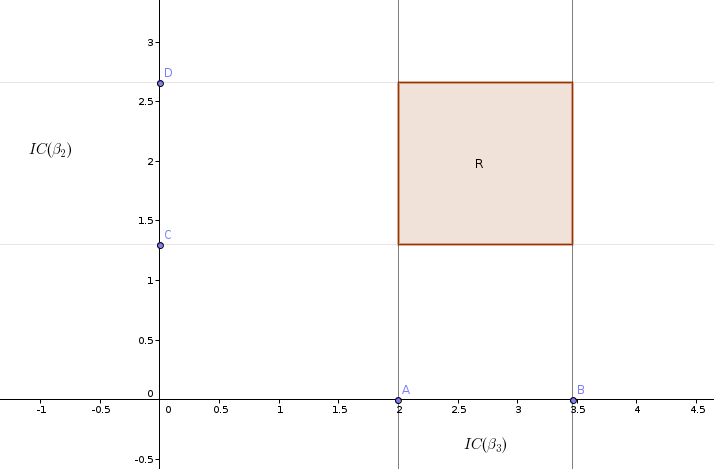
\includegraphics[scale=0.5]{img/confianzamultivariantemal.png}
\end{center}

 Pero al no ser independientes, no estamos teniendo en cuanto las correlaciones, la información que me da saber $β_1$ para saber $β_3$.

\begin{center}
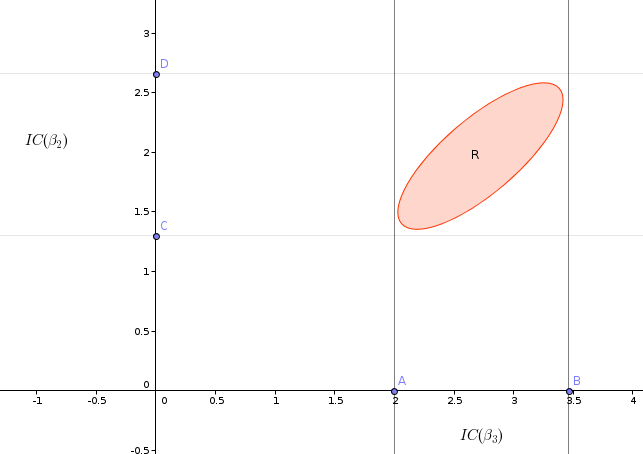
\includegraphics[scale=0.5]{img/confianzamultivariantebien.png}
\end{center}

\paragraph{Vamos a ello formalmente:}
\newcommand{\bpp}{β_{(p)}}
\newcommand{\hbpp}{\hat{β}_{(p)}}
\newcommand{\fpnk}{F_{p,n-k-1}}
Sea $β_{(p)}$ un conjunto de coeficientes de $β$. Sea $\hbpp$ el correspondiente subconjunto de estimadores.

Sea $Q_q$ la submatriz de $(X'X)^{-1}$ cuyas filas y columnas corresponden a las coordenadas del vector $\bpp$.

\[\hbpp \equiv N_p \left( \bpp, σ^2Q_p \right)\]

Si este es nuestro estimador, vamos a estandarizarlo (utilizando propiedades del tema 1).

\[
\frac{(\hbpp - \bpp)'Q_p^{-1}(\hbpp - \bpp)}{σ^2}\equiv \chi^2_p
\]

Tenemos el problema de que no conocemos $σ$ y tenemos que estimarlo. Para ello, vamos a seguir un proceso parecido a \ref{Cuentas:largas}. Para ello necesitamos:

\begin{defn}[Distribución $F_{n,m}$]

\[
F_{n,m} \equiv \frac{\chi^2_m / m}{\chi^2_n / n}
\]

Es muy habitual que aparezca la $F$ al comparar varianzas.
\end{defn}

Sabiendo lo que es una $F$, vamos a estudiar qué ocurre al cambiar $σ$ por $S_R$

\[
\frac{(\hbpp - \bpp)'Q_p^{-1}(\hbpp - \bpp)}{S_R^2} = \frac{\frac{(\hbpp - \bpp)'Q_p^{-1}(\hbpp - \bpp)}{σ^2}}{\frac{S_R^2}{σ^2}}
\]

En el numerador tenemos una $\chi^2_p$, pero nos faltaría dividir por los grados de libertad para tener una $F$, entonces:

\[
\frac{\frac{(\hbpp - \bpp)'Q_p^{-1}(\hbpp - \bpp)}{pσ^2}}{\frac{S_R^2}{σ^2}} = \frac{\chi^2_p/p}{\chi^2_{n-k-1}/n-k-1} \equiv F_{p,n-k-1}
\]

\paragraph{Conclusión}

\[
\frac{(\hbpp - \bpp)'Q_p^{-1}(\hbpp - \bpp)}{pS_R^2} \equiv F_{p,n-k-1}
\]
\[
1-α = P\left( (\hbpp - \bpp)'\left(S_R^2Q_p\right)^{-1}(\hbpp - \bpp) \leq p F_{p,n-k-1}\right)
\]

Esto nos da un elipsoide de confianza, es decir, sabemos que caerá en la región del elipsoide con probabilidad $1-α$:

\begin{figure}[hbtp]
	\centering
	\inputtikz{elipsoide_confianza}
\end{figure}

\begin{example}
Vamos a querer contrastar si son iguales los coeficientes $β_2,β_3$ las variables ``Income'' y ``Miles''. La hipótesis es: $H_0 : β_2=β_3$ a nivel $α=0.05$

Aquí damos los datos necesarios para completar (en la realidad, los obtendremos de $R$:
\[
S_R^2Q_{(2)} = \begin{pmatrix} 259.45&7.89\\7.89&2.52 \end{pmatrix}
\]

Vamos a proceder al contraste. Construimos el estadístico para construir la región de rechazo:

\[
t = \frac{|\hat{β}_2 - \hat{β}_3|}{E.T.(\hat{β}_2-\hat{β}_3)} = \frac{1.725}{15.687} \not \ge t_{45;0.025}
\]

Por tanto no podemos rechazar la hipótesis nula de que $β_2=β_3$.

El error típico se ha calculado es:
\[\sqrt{\var{\hat{β}_2-\hat{β}_3}} = \sqrt{(1,-1) S_R^2Q_p (1,-1)} = 15.687\]
Y los 45 grados de libertad los obtenemos de $R$.

\end{example}

\subsubsection{Predicción}

\paragraph{Confianza de $Y_0 | X_0$}
\[
m_0 = E(Y_0 | X_0) = β'X_o \to \hat{m}_0 \equiv N\left( β'X_0 , σ^2X'_0(X'X)^{-1}X_0 \right)
\]
Ahora ya podemos calcular el intervalo de confianza para $Y_0$ dado un vector $X_0$.

\[
\left[ \hat{Y}_0 \mp t_{n-k-1;\frac{α}{2}} S_R\sqrt{X_0'(X'X)^{-1}X_0} \right]
\]


\paragraph{Predicción de $Y_0$}

\[
\left[ \hat{Y}_0 \mp t_{n-k-1;\frac{α}{2}} S_R\sqrt{1+X_0'(X'X)^{-1}X_0} \right]
\]

\section{Análisis de la varianza (ANOVA)}

\subsection{Conceptos previos}
Las variabilidades se miden mediante la suma de cosas al cuadrado. Vamos a definir 3 sumas de cuadrados:

\begin{defn}[Suma de cuadrados\IS total]
Medimos la variabilidad total con:
\[SCT = \sum_{i=1}^n (Y_i - \gor{Y})^2\]

Esta suma de cuadrados, mide la variabilidad ``real'' de los datos. Aquí no hay ningún modelo.
\end{defn}

\begin{defn}[Suma de cuadrados\IS de la regresión]
Medimos la variabilidad explicada por el modelo con:

\[SCR = \sum_{i=1}^n (\hat{Y_i} - \gor{Y})^2\]

Esta suma de cuadrados, mide la variabilidad según el modelo. En caso de $SCT = SCR$, tendríamos que el modelo es perfecto.
\end{defn}



\begin{defn}[Suma de cuadrados\IS total]
Medimos la variabilidad no explicada.

\[SCE = \sum_{i=1}^n (Y_i - \hat{Y_i})^2\]

\end{defn}


Intuitivamente, si el modelo estuviera bien construido sería razonable esperar que $SCT = SCR + SCE$.
Vamos a complicarnos la vida y utilizar la interpretación geométrica para ver que esa relación es cierta:


\paragraph{SCT vectorialmente}

\[
SCT = ||Y - \gor{Y}1_n||^2
\]

Vamos a ver una manera complicada de entender la media muestral: Proyección de un vector al espacio de proyección de los vectores con las mismas coordenadas. ¿Esto a qué viene?
\[
\gor{Y}1_n = \frac{1}{n}1_n1'_nY = MY
\]
Siendo \[M = \begin{pmatrix}\frac{1}{n} & ... & \frac{1}{n} \\ \vdots & \ddots & \vdots \\ \frac{1}{n} & ... & \frac{1}{n}\end{pmatrix}\]

Entonces, podemos construir:

\[
SCT = ||Y - \gor{Y}1_n||^2  = || Y-MY||^2 = ||(I-M) Y||^2 = Y'(I-M)Y
\]

\paragraph{SCR vectorialmente}
\[
SCR = || HY-MY||^2 = Y'(H-M)'(H-M)Y
\]

Necesitamos ver que $H-M$ es una matriz simétrica e idempotente. Recordamos que $H$ es la matriz de proyección sobre $\mathcal{V}$.

\[
(H-M)(H-M) = HH - MH - HM + MM \overset{(1)}{=} H - M
\]
$(1)$ sabemos que $HH = H$ y $MM=M$ porque ambas son idempotentes. Pero para tener una $M$ restando, necesitaríamos $MH = HM = M$.

Geométricamente, es fácil ver que $HM=M$. Esto se debe a que $M$ es la proyección sobre un espacio vectorial más pequeño e incluido en $H$, entonces al haber proyectado con $M$, volver a proyectar con $H$ no nos cambia nada.

Por otro lado, $MH = M$. En este caso, primero proyectamos en el subespacio grande, pero como acabamos proyetando sobre el pequeño.

\paragraph{Ejercicio: } Demostrar algebraicamente $MH=HM=M$.

\paragraph{SCE vectorialmente}
\[SCE = ||HY-H||^2 = Y'(I-H)Y\]

\begin{prop}[Relación de las sumas de cuadrados]
\[SCT = SCR + SCE\]
\end{prop}

\begin{proof}
\[SCT = Y'(I-M)Y = Y'(H-M+I-H)Y = Y'(H-M)Y + Y'(I-H)Y = SCR + SCE\]
\end{proof}

\begin{figure}[hbtp]
	\centering
	\inputtikz{relacion_SCE_SCT_SCR}
	\caption{Representación de los vectores $SCE,SCT,SCR$ sobre el espacio vectorial $\mathcal{V}$.}
\end{figure}

\subsubsection{Contraste de la regresión}
Queremos contrastar $H_0 : β_1 = ... = β_n = 0$.

La idea intuitiva es que si $SCR$ es muy pequeño, tenemos poca variabilidad explicada sería razonable que aceptáramos la hipótesis nula de que las variables regresoras no influyen mucho.

Por el contrario, si $SCR$ es muy \textbf{grande}, tenemos mucha variabilidad explicada, por lo que la hipóteis nula no es muy razonable y deberíamos \textbf{rechazar}. Por el contrario, si $SCR$ es \textbf{pequeña} aceptamos $H_0$.


Para ello, es imprescindible definir ``grande'' y ``pequeño''. Deberían tener las mismas unidades. No puede ser que por cambiar de unidades afecte a la validez de la hipótesis. Además, necesitamos saber la distribución de $SCR$ bajo la hipótesis nula.

\begin{prop}[Distribución SCR en $H_0:∀i\;β_i=0$]

\[
\frac{SCR}{σ^2} \equiv \chi^2_{k}
\]
\end{prop}
\begin{proof}
Tenemos $SCR = Y'(H-M)Y$, una forma cuadrática, teniendo $H-M$ simétrica e idempotente (por construcción).

Ahora, para poder aplicar la proposición del tema 1, necesitamos $µ'(H-M)µ = 0$.

Sabemos que $µ$, bajo $H_0$ tiene todas sus coordenadas iguales, con lo que está en el subespacio $1_n$, por lo que las proyecciones sobre $V$ y sobre $1_n$ de $µ$ serán $µ$. Esto quiere decir que:
\[ Hµ = µ \;\;\; Mµ = µ \to (H-M)µ=0\]


Por otro lado, los $k$ grados de libertad:
\[
gl = \rg(H-M) = \tr(H-M) = \tr(H) - \tr(M) = (k+1)-1 = k
\]

Esto se debe a que la traza de una matriz de proyección es la dimensión del espacio en el que proyectamos.

\end{proof}

As usual, como no conocemos $σ^2$, en la práctica utilizamos:
\begin{prop}
\label{prop:estad_contr_regresion}
\[
\frac{SCR}{k·S_R^2} = \frac{\displaystyle\frac{SCR}{k}}{\displaystyle\frac{SCE}{n-k-1}} = \frac{\chi^2_k}{\chi^2_{n-k-1}}\sim F_{k;n-k-1}
\]
\end{prop}
\begin{proof}
Para ello necesitamos que $SCR$ y $SCE$ sean independientes. Son normas al cuadrado de vectores ortogonales. Estadísticamente, la ortogonalidad de vectores normales se traduce en independencia.

Para ello, vamos a ver que el producto de las matrices es 0 (utilizando la propiedad \ref{prop:tema1_pepino})

\label{prop:SCRIndepSCE}
\[
(H-M)(I-H) = H-H-M+\underbrace{MH}_{M} = 0
\]
Sabemos que $MH=M$ por que, por un lado es proyectar en $V$ después de haber proyectado en un subespacio de $V$ ($1_n$) y en el otro, tenemos la proyección directamente sobre $1_n$.

\end{proof}

\subsubsection{Tabla anova}
Para este caso, vamos a construir la tabla \concept{ANOVA} (análisis de la varianza)

Este es el ejemplo de una tabla ANOVA simple:
\begin{center}
\begin{tabular}{c|ccccc}
Fuente de variación & SC & gl & CM & F & p-valor\\\hline
Explicada & SCR & k & $\frac{SCR}{k}$ & $\displaystyle\frac{SCR/k}{SCE/(n-k-1)}$ & ...\\
No explicada & SCE & n-k-1 & $\frac{SCE}{n-k-1}$ & ... & ...\\\hline
total & & & &
\end{tabular}
\end{center}

\subsubsection{Coeficiente de determinación}
\begin{defn}[Coeficiente\IS de determinación]
Es una medida de la bondad del ajuste en el modelo de regresión múltiple \[R^2 = \frac{SCR}{SCT}\]
\end{defn}

\paragraph{Propiedades:}
\begin{itemize}
	\item $R^2≤1$ (ya que un cateto siempre es menor o igual que la hipotenusa)
	\item Vamos a ver los casos extremos.
	\subitem $R^2 = 1$ quiere decir que existe una relación lineal exacta debido a que \[R^2 = 1\implies SCR = SCT \implies SCE=0 \implies ∀i\;e_i=0\]

	De hecho, podemos interpretar $R^2$ como un coeficiente de correlación múltiple entre las $k$ variables $X$ y la $Y$.
	\subitem $R^2 = 0$ quiere decir que no existe una relación lineal debido a que \[R^2 = 0 \implies Σ(\hat{Y_i} - \gor{Y})^2 = 0 \implies \hat{Y_i}=\gor{Y} \implies \text{ ninguna X aporta información para calcular Y}\]
	\item Se verifica que el estadístico $\displaystyle F = \frac{R^2}{1-R^2} \frac{n-k-1}{k}$
	\begin{proof}
		Esta identidad se obtiene inmediatamente utilizando la definición de $R^2$. Se deja como ejercicio para quien quiera escribirse la cuenta.
	\end{proof}
\end{itemize}

Este coeficiente es útil en el contraste que estudiábamos anteriormente $H_0: ∀i\;β_i = 0$. En este contraste, es equivalente para rechazar o aceptar \begin{itemize}
	\item $SCR$ es ``grande''.
	\item $F$ es ``grande''.
	\item $R^2$ se aproxima a 1.
\end{itemize}


El coeficiente de determinación para comparar distintos modelos de regresión entre sí tiene el siguiente inconveniente:
Siempre que se añade una nueva variable regresora al modelo, $R^2$ aumenta, aunque el efecto de la variable regresora sobre la respuesta no sea significativo. ¿Porqué aumenta $R^2$? Porque la dimensión de $V$ aumenta provocando que disminuya $SCE$ (por algo que me he perdido) y al disminuir $SCR$, aumenta $SCR$ (porque su suma es constante) y aumenta $R^2$.



Por ello, definimos:


\begin{defn}[Coeficiente de determinación ajustado]
\[\gor{R}^2 = r^2 = 1 - \frac{SCE/(n-k-1)}{SCT/(n-1)}\]
Esta nueva definición penaliza un aumento de las variables utilizadas. De esta manera, al aumentar $K$, sabemos que $R^2$ aumenta pero $\gor{R}^2$ puede aumentar o no. Depende de si la ganancia de información es mayor que la penalización de añadir más variables.
\end{defn}

Vamos a ver un ejemplo realmente ilustrativo.
\begin{example}

Vamos a utilizar el modelo de regresión múltiple para ajustar el grado del polinomio.

El proceso a seguir podría ser: voy calculando $R^2$ para todos los grados que vaya teniendo hasta que tenga $R^2 = 1$, que hace que podamos explicar toda la varianza con estos datos.


Al aumentar el grado, obtenemos polinomios cada vez mejores (para estos datos).

\begin{center}
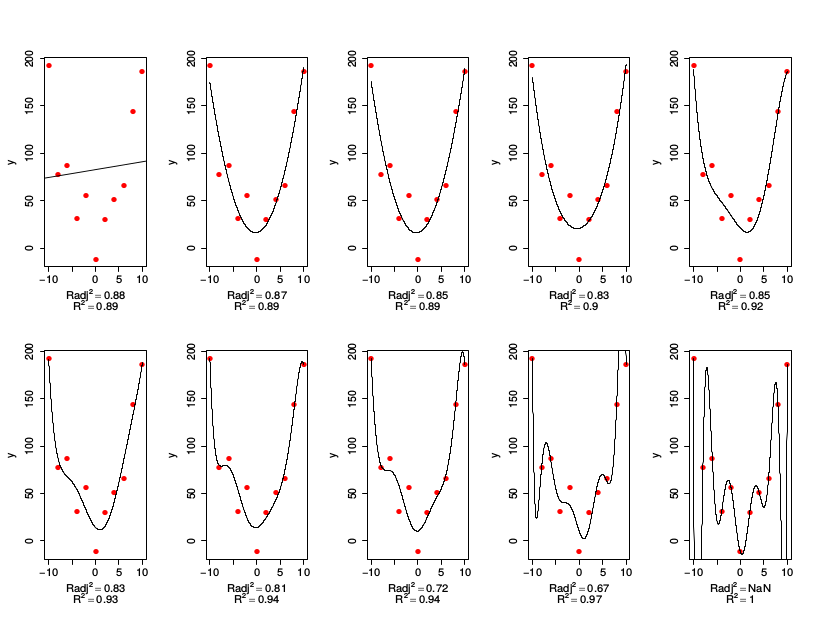
\includegraphics[scale=0.45]{img/RvsRAdj.png}
\end{center}

Si tomáramos una nueva muestra de datos, el modelo que tiene $R^2=1$ sería una mierda muy probablemente. En este caso, sería una bazofia absoluta ya que los datos han sido generados parabólicamente. Es por ello que el modelo con mayor $\gor{R}^2$ es el segundo.

\end{example}


\begin{example}

Si un modelo es demasiado simple, tendremos muy poca varianza pero mucho sesgo. Por el otro lado, si el modelo es demasiado complejo, tenemos mucha varianza pero muy poco sesgo. Vamos a verlo con un ejemplo:

\begin{center}
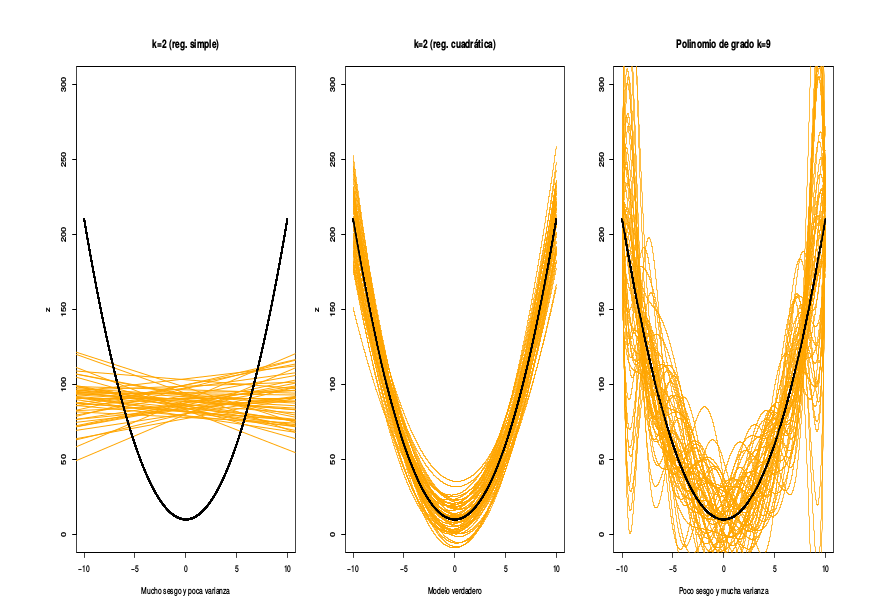
\includegraphics[scale=0.45]{img/ModeloSimpleVsModeloComplejo.png}
\end{center}

En este ejemplo, el primer caso, demasiado simple tiene muy poca varianza. Todas las pendientes son similares, pero por el contrario, siempre estimamos mal.

En el tercer caso, si cogemos un único polinomio, vemos que es un poco malo, pero si tomáramos la media de todos ellos, más o menos se asemeja bastante a la parábola, es decir, la esperanza es el valor esperado con lo que el sesgo sería muy pequeño. Por el contrario, cada polinomio es de su padre y de su madre, es decir, tiene mucha varianza estimar así.
\end{example}

\begin{example}
Vamos a calcular el coeficiente de determinación para el caso de regresión simple:

\[R^2 = \frac{SCR}{SCT} = \frac{\sum(\hat{Y}_i - \gor{Y})}{} = ... \frac{\hat{β}_1^2S_{xx}}{S_{yy}} = r^2\]

es decir, el coeficiente de determinación en regresión múltiple coincide con el coeficiente de determinación ajustado.

\end{example}
\subsection{Contrastes de hipótesis lineales}

Queremos contrastar $H_0 : Aβ = 0$, donde $A$ es una matriz $p×(k+1)$ con $\rg(A) = p < k+1$.

\begin{example}
En el modelo
$Y_i = β_0 + β_1x_{i1} + β_2x_{i2} +β_3x_{i3} + ε_{i}$
queremos contrastar

\[
H_0 : β_1 = β_2\; β_0=0 \dimplies Aβ = 0 \to A = \begin{pmatrix}
0&1&-1&0\\
1&0&0&0
\end{pmatrix}
\]
\end{example}

\begin{defn}[Modelo\IS reducido ($M0$)]
Es el modelo resultante al imponer las restricciones de $H_0$.
\end{defn}
\begin{example}
Tomando el \concept{Modelo\IS completo} del ejemplo anterior
\[\left.\begin{array}{c} Y_i = β_0 + β_1x_{i1} + β_2x_{i2} +β_3x_{i3} + ε_{i}\\H_0 : β_1 = β_2\; β_0=0\end{array}\right\} \to Y_i = β_1(x_{i1} + x_{i2}) + β_3x_3 + ε_i
\]

El modelo simple es $Y_i = β_1(x_{i1} + x_{i2}) + β_3x_3 + ε_i$
\end{example}

\paragraph{Cómo elegir un modelo}

Nos podemos plantear qué modelo podemos elegir. La idea sería elegir siempre lo simple, pero tenemos que ver cuánto perdemos con la simplificación. A esto se le denomina \concept{Principio\IS de incremento relativo de la variabilidad}

\begin{figure}[hbtp]
	\centering
	\inputtikz{incremento_var_relativa}
	\caption{interpretação geométrica de erro inexplicável no modelo completo e reduzido, em que $\mathcal{V}_0$ é o espaço vectorial em que as estimativas são obtidas modelo reduzida (do exemplo $dim(\mathcal{V}_0)=2$, $dim(\mathcal{V})=4$).}
\end{figure}

La idea es que $SCE_0 > SCE$. Geométricamente, vemos que $SCE_0$ es la hipotenusa y $SCE$ es un cateto. Por otro lado, la variabilidad no explicada de un modelo simple siempre va a ser menor que la $SCE$ de un modelo complejo para los mismos datos.

Entonces la idea sería rechazar $H_0$ cuando se pierda mucho al considerar $M0$ en lugar de $M$, es decir cuando $SCE_0 - SCE$ sea muy grande. Para evitar problemas generados por cambios de escala, tomamos \[\frac{SCE_0 - SCE}{SCE}\]

¿Y esto que distribución tiene? ¿Cómo podemos definir ese ``suficientemente grande''? Las sumas de cuadrados ($SCE$) son $\chi^2$ y el cociente de $\chi^2$'s es una $F$. Vamos a estudiarlo formalmente:


\paragraph{Distribución de $(SCE_0 - SCE)/SCE$}

Sea $X$ la matriz de diseño del modelo reducido correspondiente. ``Hat matrix'' es $H_0 = X_0(X_0'X_0)^{-1}X_0'$, donde tenemos $\rg(H_0) = \tr(H_0) = k+1-p$. El rango es la traza porque es una matriz de proyección y eso es lo que debería ser debido a ........

Vamos a construir el estadístico:

\[
SCE_0 - SCE = Y'(I-H_0)Y - Y'(I-H)Y = Y'(H-H_0)Y
\]

Vamos a ver si $H-H_0$ es simétrica e idempotente, teniendo que $H_0H_0 = H_0$, por ser una matriz de proyección.
\[
(H-H_0)(H-H_0) = H - H_0H - HH_0 + H_0 = H_0
\]

Aquí tenemos que  $H_0H = HH_0 = H_0$ por el mismo argumento que en \ref{prop:SCRIndepSCE} Ambas son matrices de proyección sobre subespacios en los que uno está contenido dentro del otro, por lo que da igual el orden en el que proyectar y además, será lo mismo que proyectar sobre el pequeño.

Ahora, necesitamos ver que $µ'(H-H_0)µ = 0$ para poder tener que $SCE_0 - SCE \sim \chi^2$. Aquí el razonamiento vuelve a ser muy parecido.
\[(H-H_0)µ = Hµ - H_0µ = µ-µ = 0\]
Proyectar $µ$ con $H$ y con $H_0$ no cambia $µ$, debido a que $µ$ está en el subespacio de proyección pequeño $V_0$. ¿Porqué sabemos que $µ∈V_0$? Porque, asumiendo $H_0$

\[
\begin{array}{lcr} \displaystyle\frac{SCE_0 - SCE}{σ^2} \overset{H_0}{\equiv} \chi^2_{p} && \displaystyle\frac{SCE}{σ^2} \equiv \chi^2_{n-k-1}\end{array}
\]

Si fueran independientes, su cociente sería una $F$. Vamos a ver la independencia utilizando \ref{prop:tema1_pepino} y utilizando que $HH = H$ y $HH_0 = H_0H = H_0$ por ser matrices de proyección.

\[(H-H_0)(I-H) = H-H_0 - H + H_0 = 0\to \text{ independientes}\]

Concluimos que
\[
\frac{(SCE_0-SCE)/p}{SCE/(n-k-1)} \overset{H_0}{\equiv} F_{p;n-k-1}
\]

Cuya región de rechazo será para un nivel $α$ será

\[
R_α = \left\{\frac{(SCE_0-SCE)/p}{SCE/(n-k-1)} > F_{p,n-k-1;α} \right\}
\]

\obs El contraste $H_0: β_1 = ... = β_k = 0$ es un caso particular de esto que hemos visto, tomando en $Aβ = 0$ la matriz $A$ como:

\[A =
\begin{pmatrix}
	\underbrace{\begin{matrix}0\\\vdots\\0\end{matrix}}_{(1)}  &
	%\begin{matrix}\vdots\\\vdots\\\vdots\end{matrix}
	I_k
\end{pmatrix}
\]
$(1)$: por $β_0$.

En este caso, el modelo reducido sería $Y_i = β_0 + ε_i$, con lo que

\[SCE_0 = \sum (Y_i-\hat{Y_i})^2 \overset{(2)}{=} \sum(Y_i - \gor{Y})^2=SCT\]

$(2)$:debido a que $Y_1,...,Y_n \sim N(β_0,σ^2)$, con lo que $\hat{β}_0 = \gor{Y}$.

Como $SCE_0 = SCT$, tenemos lo que ya habíamos obtenido:
\[SCE_0 = SCT \to {SCE}_0 -SCE = SCT - SCE = SCR\]


\subsubsection{Explicación de la tabla ANOVA}

$R$ siempre está comparando 2 modelos, el reducido y el completo.Vamos a entenderla por inducción matemática:

En la primera fila, el modelo completo es el que incluye la primera variable y el modelo reducido es el que no incluye ninguna.

El la fila $n$, el modelo completo es el que incluye las $n$ variables, y el modelo reducido es el que incluye las $n-1$ variables.


% % % TODO: como texto cuando me lo pase JoseR.
\begin{center}
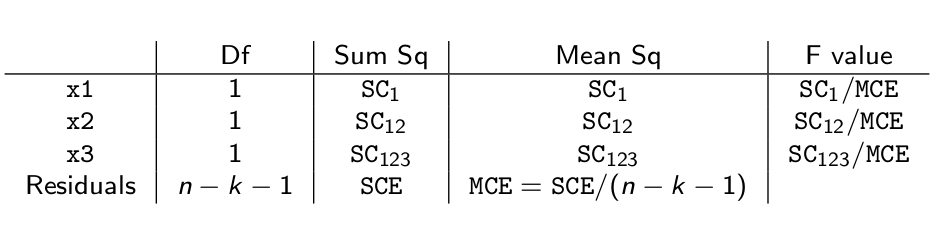
\includegraphics[scale=0.4]{img/TablaAnovaGeneral.png}
\end{center}



Es importante darse cuenta que los números de la columna $SumSq$ dependen del orden de las variables, ya que no es lo mismo pasar de no tener variables a tener la primera variable (que puede no influir nada) a tener la segunda (que puede ser tremendamente explicativa).

\textbf{Sin embargo,} la suma es \textbf{constante}. Vamos a verlo
\begin{proof}
\[
\begin{array}{cccccc}
SC_1 &+ &SC_{12} &+ &SC_{123} &= \\
(SCE_0 - SCE_1) &+ &(SCE_1 - SCE_{12}) &+ &(SCE_{12} - SCE_{123})&=\end{array}  \]
\[ SCE_0 - SCE_{123} = SCT - SCE = SCR\]
\end{proof}


\begin{example}
Vamos a ver una tabla anova normal, con los datos del consumo de combustible en EEUU:

\begin{lstlisting}[style=mystyle]
reg <- lm(FuelC ~ Drivers+Income+Miles+MPC+Tax, data=fuel2001)
anova(reg)

Response: FuelC
          Df     Sum Sq    Mean Sq   F value    Pr(>F)
Drivers    1 3.5301e+14 3.5301e+14 2273.2167 < 2.2e-16 ***
Income     1 6.7563e+11 6.7563e+11    4.3507 0.0426945 *
Miles      1 2.1698e+12 2.1698e+12   13.9723 0.0005216 ***
MPC        1 5.2927e+11 5.2927e+11    3.4082 0.0714577 .
Tax        1 4.1208e+11 4.1208e+11    2.6536 0.1102978
Residuals 45 6.9882e+12 1.5529e+11
---
\end{lstlisting}

Vemos que el $p-valor$ de la última variable es $0.1102978$. Si vamos al análisis de regresión múltiple hecho al principio de la sección (\ref{example:fuel2001}) vemos que el p-valor de $Tax$ (nuestra última variable) es $0.110298$. ¿Casualidad o causalidad?

La última columna de la fila $n$ es el p-valor del contraste $β_n = 0$, tomando el modelo que tiene las $β_0,...,β_{n-1}$. En el caso de la última fila, tenemos el p-valor de si $β_{ultimo} = 0$ en el modelo que incluye todas las demás variables. Este contraste es equivalente al que hacíamos en regresión múltiple para contrastar si $β_j = 0$. Podemos comprobar que los p-valores coinciden (0.11).

\end{example}



\begin{example}
Vamos a ver ahora el contraste de si podemos utilizar el modelo simple frente al complejo.

\begin{lstlisting}[style=mystyle]

regsimple <- lm(FuelC ~ Drivers,data=fuel2001)
anova(regsimple, reg)

Model 1: FuelC ~ Drivers
Model 2: FuelC ~ Drivers + Income + Miles + MPC + Tax
  Res.Df        RSS Df  Sum of Sq      F    Pr(>F)
1     49 1.0775e+13
2     45 6.9882e+12  4 3.7868e+12 6.0962 0.0005231 ***
---
\end{lstlisting}

Es de recibo comentar que: $RSS = SCE$

Por otro lado, son 4 grados de libertad porque imponemos 4 restricciones del modelo compuesto para el modelo simple (4 coeficientes nulos 0).


El p-valor obtenido, al ser tan pequeño nos dice que la ganancia de información es suficientemente grande como para tener que rechazar el modelo simple.

\end{example}

\subsubsection{Análisis de influencia}

En esta subsección vamos a estudiar cuánto de influyente puede ser una observación. En el caso de regresión simple, teníamos que algunos datos atípicos podían desviar mucho la recta (ver \ref{ej:reg_simple}). ¿Qué ocurre en regresión múltiple? Aquí no podemos hacer razonamientos geométricos para entenderlo, pero es un tema importante que tratar.


Vamos a estudiarlo utilizando un ejemplo en el que queremos saber la cantidad de cierto medicamento en el hígado de una rata, tras recibir una dosis oral. La dosis recibida fue de 40 mg por kg de peso corporal. Tras cierto tiempo se sacrifican las ratas y se mide la cantidad de medicamento en su hígado.

Tenemos 19 observaciones, y tres variables regresoras (peso de la rata, peso del hígado y dosis recibida) para la variable respuesta (Proporción de dosis en el hígado)


Vamos a ver contrastando con regresión simple cada $β_i = 0$. Estos son los resultados obtenidos:
\begin{center}
\begin{tabular}{ccccc}
&Estimate&Std. Error&t value&Pr(>|t|)\\\hline
(Intercept)&0.1962346&0.2215825&0.886&0.388\\
BodyWt&0.0008105&0.0012862&0.630&0.537
\end{tabular}

\begin{tabular}{ccccc}
&Estimate&Std. Error&t value&Pr(>|t|)\\\hline
(Intercept)&0.22037&0.13573&1.624&0.123\\
LiverWt&0.01471&0.01718&0.856&0.404
\end{tabular}

\begin{tabular}{ccccc}
&Estimate&Std. Error&t value&Pr(>|t|) \\\hline
(Intercept)&0.1330&0.2109&0.631&0.537\\
Dose&0.2346&0.2435&0.963&0.349
\end{tabular}
\end{center}
Vemos que los $p-valores$ son muy grandes, con lo que no podemos rechazar $β_i = 0$ y no debería haber relación entre la variable respuesta a partir de la regresora. Además, podemos corroborarlo gráficamente:

\begin{center}
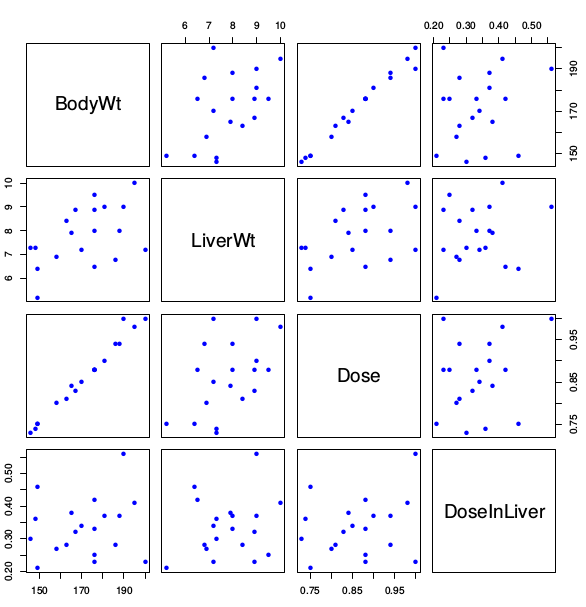
\includegraphics[scale=0.6]{img/DiagramaRatas.png}
\end{center}

Aparentemente no hay relación entre la respuesta y las regresoras. \textbf{¿Y haciendo regresión múltiple?} Tal vez contrastando $β_1 = ... = β_3 = 0$ obtengamos otra cosa (aunque sería de esperar que no).

\begin{tabular}{ccccc}
&Estimate&Std. Error&t value&Pr(>|t|)\\\hline
(Intercept)&0.265922&0.194585&1.367&0.1919\\
BodyWt&-0.021246&0.007974&-2.664&\textcolor{red}{0.0177}\\
LiverWt&0.014298&0.017217&0.830&0.4193\\
Dose&\textcolor{red}{4.178111}&1.522625&2.744&\textcolor{red}{0.0151}
\end{tabular}

Hay unos cuantos valores extraños. ¿Ahora resulta que $BodyWt$ y $Dose$ (que además son prácticamente la misma variable, ya que existe una gran correlación entre ellas) si son influyentes? Pero si antes no lo eran... Además, el término independiente de $Dose$ es tremendamente distinto al anterior\footnote{\textbf{Se deja como ejercicio para profundizar: }\textit{Demostrar que los $β_i$ de un modelo de regresión simple son iguales a los $β_i$ de cada regresión simple por cada variable regresora si éstas son independientes (o incorreladas).}}. ¿Cómo puede ser esto posible? \textbf{La paradoja se produce por un dato atípico.} Vamos a verlo, pero para ello necesitamos un par de medidas, para poder entender lo atípico del dato.




\begin{defn}[Potencial en un punto]
El potencial (\concept{leverage}) de un punto es el correpondiente $h_i$ de la matriz de diseño $X$.
\end{defn}

Los potenciales definen las varianzas, ya que
\[\var{e_i} = σ^2(1-h_i)\]
\begin{proof}
Esto se debe a la distribución de los residuos.

Recordamos $e = Y - \hat{Y} = (I-H)Y$. Como $Y\equiv N(Xβ,σ^2I_n)$, tenemos:

\[
e \equiv N\left(0,(I-H)σ^2I_n(I-H)'\right) \equiv N(0,σ^2(I-H))
\]
\end{proof}

Además, este potencial está tremendamente relacionado con la distancia de Mahalanobis $\dist_M$:
\[h_i = \frac{1}{n} \frac{1}{n-1}\dist_M(x_i,\gor{x})\]

Este potencial mide numéricamente la influencia de un único punto. Para valores $>0.5$, el libro (sin justificación teórica) sugiere preocuparse porque tal vez sea un dato atípico. Otra manera (más natural) de medir la influencia, es recalcular el modelo eliminando el dato. Si cambia mucho, el dato es influyente. Si no cambia nada, el dato no es influyente. Esta es la idea que hay detrás de la \textbf{Distancia de Cook}.

\begin{defn}[Distancia\IS de Cook]
La distancia de Cook mide cómo cambia el vector de estimadores $\hat{β}$ cuando se elimina cada observación.

Para ello, se utiliza la distancia de Mahalanobis (estandarizada) entre $\hat{β},\hat{β_i}$.

Recordando la matriz de covarianzas de $\hat{B} = S_R^2(X'X)^{-1}$, entonces:

\[D_i = \frac{[\hat{β} - \hat{β_i}]' (X'X) [\hat{β} - \hat{β_i}]}{(k+1)S_R^2} \]
\end{defn}

\paragraph{Propiedades}
\begin{itemize}
	\item ¿Cuándo es grande esta distancia? Lo que se hace es calibrarlo comparando con $F_{k+1,n-k-1;α}$. En general $D_i>1$ suele ser relevante.
	\item Se puede calcular de una manera más simple utilizando los valores ajustados:
	\[D_i = \frac{\sum_j=1^n \left(\hat{Y}_j(i) - \hat{Y}_j\right)^2}{(k+1)S_R^2}\]
	\item Y también está relacionado con el potencial y los residuos.
	\[
		D_i = \frac{1}{k+1}r_i^2 \frac{h_i}{1-h_i}
	\]
	donde $r_i = e_i/(S_R\sqrt{1-h_i})$, los residuos estandarizados.
\end{itemize}



En el ejemplo (\ref{ej:reg_simple}), tanto el punto rojo como el verde tienen un alto potencial, pero el rojo tiene una distancia de Cook mucho menor, ya que no es muy atípico  (en tanto en cuanto el modelo se ajusta bien a ese dato). En cambio, el punto verde tiene una distancia de Cook mucho mayor.

Volviendo al ejemplo de las ratas, vamos a ver porqué esa paradoja de los $β_i$ distintos en regresión simple que en compuesta.



Calculando los potenciales y las distancias de Cook, vemos que:
\begin{center}
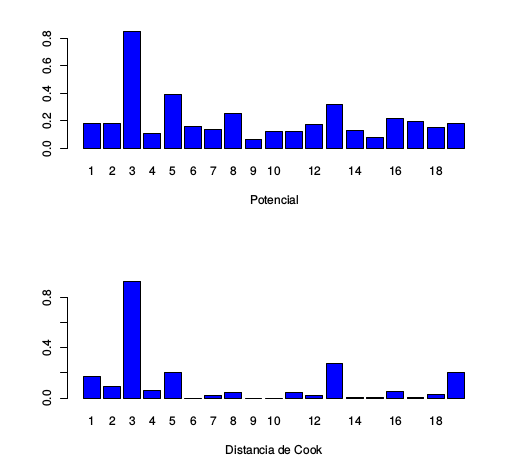
\includegraphics[scale=0.75]{img/CookVsPotencial.png}
\end{center}

La rata 3 es como muy rara, ya que tiene un potencial y una distancia de Cook muy altos. Vamos a pintarla en rojo, para que veamos de qué dato estamos hablando:

\begin{center}
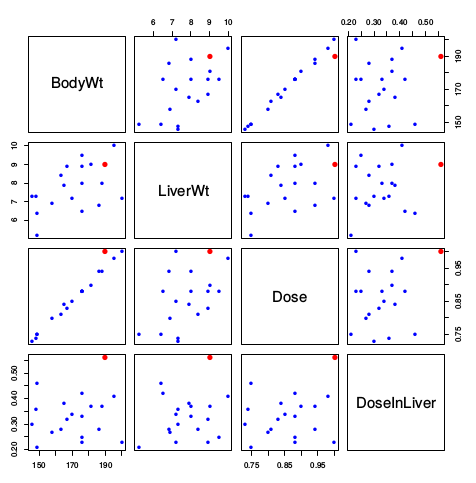
\includegraphics[scale=0.6]{img/DiagramaRatasRojo.png}
\end{center}

Vemos que algo raro sí parece, pero a simple vista no parece que podamos juzgar. Esta es la utilidad de estas medidas. Vamos a eliminar esa rata y recalcular los p-valores:

\begin{center}
\begin{tabular}{ccccc}
Coefficients&Estimate&Std. Error&t value&Pr(>|t|)\\\hline
(Intercept)&0.311427&0.205094&1.518&0.151\\
BodyWt[-3]&-0.007783&0.018717&-0.416&0.684\\
LiverWt[-3]&0.008989&0.018659&0.482&0.637\\
Dose[-3]&1.484877&3.713064&0.400&0.695
\end{tabular}
\end{center}

\paragraph{Conclusión}
Una única observación hace que cambien totalmente las conclusiones respecto a si las variables son o no significativas.


\subsection{Variable regresora cualitativa}

Este es un tema que da para libros enteros. También se llama ``diseño de experimentos''. Nosotros vamos a ver el \concept{Modelo\IS unifactorial}, un caso concreto del tema para entender el fundamento matemático que hay detrás. Todo lo demás en lo que se profundiza en los libros son casos concretos.

Vamos a verlo con el siguiente ejemplo:

En un estudio para comparar la eficacia de tres fertilizantes se utiliza
cada uno de ellos en 10 parcelas (asignando aleatoriamente cada parcela
a uno de los tres fertilizantes) y posteriormente se registra el peso en
toneladas de la cosecha resultante en cada parcela. Los datos son:

\begin{center}
\begin{tabular}{|c|ccccccccccc|}
\hline
	Fert. 1 & 6.27 & 5.36 & 6.39 & 4.85 & 5.99 & 7.14 & 5.08 & 4.07 & 4.35 & 4.95\\
	Fert. 2 & 3.07 & 3.29 & 4.04 & 4.19 & 3.41 & 3.75 & 4.87 & 3.94 & 6.28 & 3.15\\
	Fert. 3 & 4.04 & 3.79 & 4.56 & 4.55 & 4.55 & 4.53 & 3.53 & 3.71 & 7.00 & 4.61\\\hline
\end{tabular}
\end{center}



Una variable explicativa cualitativa se llama factor. Los valores que toma se llaman niveles. En este modelo los niveles son los distintos tratamientos que aplicamos a las unidades experimentales. En el ejemplo tenemos un factor (el tipo de fertilizante) que se presenta en tres niveles o tratamientos, que se aplican a las unidades experimentales (las parcelas).


\paragraph{Notación}
\begin{itemize}
\item \textbf{k} es el número de niveles del factor (en este caso 3). En las transparencias se le denomina $I$.
\item $Y_{ij}$, donde $i$ es el nivel y $j$ es la unidad dentro del nivel.
\item $\gor{Y_{1·}}$ es la media del nivel $1$ (recordamos que $\gor{Y}_{·j}$ sería la media de la columna).
\item De esta manera, $\gor{Y_{··}}$ es la media global de todos los datos.
\end{itemize}

Con esto, podemos entender los datos de la tabla:

\begin{center}
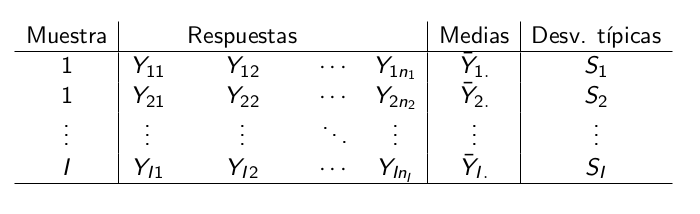
\includegraphics[scale=0.6]{img/ModeloUnifactorial.png}
\end{center}


\subsubsection{Modelo unifactorial}

\[Y_{ij} = µ_i + ε_{ij}\]

donde
\begin{itemize}
	\item $µ_i$ es el nivel medio de la respuesta para el nivel $i$ del factor.
	\item $ε_{ij}$ es la variable de error que recoge el resto de variables que
influyen en la respuesta.
	\subitem $ε_{ij} \overset{iid}{\sim} N(0,σ^2) \to Y_{ij} \equiv N(µ_i,σ^2)$.
	\subitem Vemos que son \textbf{homocedásticas}
\end{itemize}

\paragraph{Modelo unifactorial como caso de la regresión múltiple}

El modelo unifactorial se puede expresar en la forma $Y = Xβ + ε$,
donde

\begin{itemize}
	\item $Y=(Y_{1,1},Y_{1,2},Y_{k,n_k})'$
	\item $β = (µ_1,...,µ_k)$
	\item $ε=(ε_{1,1},ε_{1,2},ε_{k,n_k})'$
\end{itemize}

Vamos a construir la matriz $X$:

\[
\begin{pmatrix}
\begin{matrix} Y_{11}\\\vdots \\Y_{1n_1}\end{matrix}\\\hline
\begin{matrix} Y_{21}\\\vdots \\Y_{2n_2}\end{matrix}\\\hline
\vdots\\\hline
\begin{matrix} Y_{k1}\\\vdots \\Y_{kn_k}\end{matrix}
\end{pmatrix}
 = 
\begin{pmatrix}
	\begin{matrix}
		1&0&0&\dots\\
		1&0&0&\dots\\
		\vdots&\vdots&\vdots&\\
		1&0&0&\dots
	\end{matrix}\\\hline
	\begin{matrix}
		0&1&0&\dots\\
		0&1&0&\dots\\
		\vdots&\vdots&\vdots&\\
		0&1&0&\dots
	\end{matrix}\\\hline 
	\vdots \\\hline
	\begin{matrix}
		0&\dots&0&1\\
		0&\dots&0&1\\
		\vdots&&\vdots&\vdots\\
		0&\dots&0&1
	\end{matrix} 
\end{pmatrix}
\begin{pmatrix} µ_1 \\ \vdots \\µ_k \end{pmatrix}
\begin{pmatrix}
	\begin{matrix} ε_{11}\\\vdots \\ε_{1n_1}\end{matrix}\\\hline
	\begin{matrix} ε_{21}\\\vdots \\ε_{2n_2}\end{matrix}\\\hline
	\vdots
	\begin{matrix} ε_{k1}\\\vdots \\ε_{kn_k}\end{matrix}
\end{pmatrix}
\]


Vamos a ver que esta matriz de diseño estima $β$ correctamente:

\[\hat{β} = (\hat{µ}_1,...,\hat{µ_n}) = \underbrace{(X'X)^{-1}}_{A}\underbrace{X'Y}_{B} =
\underbrace{\begin{pmatrix}
1/n_1 & 0 & \hdots & 0\\
0 	& 1/n_2 & \hdots & 0\\
\vdots & & \ddots & \vdots\\
0 & 0 & 0 & 1/n_k
\end{pmatrix}}_{A}\underbrace{
\begin{pmatrix}
Y_{1·}\\
Y_{2·}\\
\vdots\\
Y_{k·}
\end{pmatrix}
}_{B} = \begin{pmatrix}
\gor{Y}_{1·}\\
\gor{Y}_{2·}\\
\vdots\\
\gor{Y}_{k·}
\end{pmatrix} = \gor{Y_{··}}
\]

\paragraph{Hipótesis} ¿Cuál es el contraste equivalente que queremos realizar?

Queremos contrastar si el fertilizante es influyente, es decir: $H_0 : µ_1 = ... = µ_k$.


\paragraph{Modelos reducido y completo}
\subparagraph{Reducido}
\[SCE_0 = \sum_i \sum_j (Y_{ij} - \gor{Y}_{··})^2 = SCT\]
\subparagraph{Completo}
\[SCE = \sum_i \sum_j (Y_{ij} - \gor{Y}_{··})^2 \overset{(1)}{=} \sum_i (n_i-1)S_i^2\]

$(1)$ ¿?¿?¿?

Teniendo esto, recordamos:
\[SCE_0 - SCE = SCT - SCE = SCR = \sum_i \sum_j (\gor{Y}_{i·} - \gor{Y}_{··})^2 = \sum n_i(\gor{Y}_{i·} - \gor{Y}_{··})^2\]


Ahora ya podemos construir la tabla ANOVA:

\begin{center}
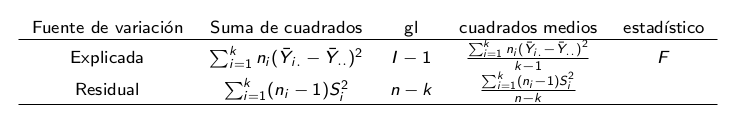
\includegraphics[scale=0.55]{img/AnovaUnifactorial.png}
\end{center}

¿Porqué $n-k$ grados de libertad? Si recordamos, ahí tendríamos $n-k-1 = n-(k+1) = n - \dim(V)$, siendo $V$ el subespacio generado por la matriz $X$. En regresión múltiple teníamos $\dim(V) = k+1$, las $k$ columnas más el término independiente. En este caso, nuestra matriz $X$ tiene rango $k$.

\begin{example}
Vamos a ver esto con los datos del ejemplo.

\begin{center}
\begin{tabular}{cccc}
Muestra & $n_i$ & $\gor{Y_{i·}}$ & $S_{i·}$\\
1 & 10 & 5.445 & 0.976\\
2 & 10 & 3.999 & 0.972\\
3 & 10 & 4.487 & 0.975
\end{tabular}
\end{center}

\[SCT = 10(5.445 - 4.644)^2 + 10(3.999 - 4.644)^2 + 10(4.487 - 4.644)^2 \simeq 10.82\]
\[SCE = 9(0.976)^2 +9(0.972)^2 +9(0.975)^2  = 25.62\]

Ahora ya podemos construir el estadístico:

\[
\frac{SCR/(k-1)}{SCE/(n-k)} = ... = 5.702
\]

Por otro lado, $F_{2,27;0.05} = 3.35$

Como el valor obtenido es mayor que el estadístico, rechazamos la hipótesis.

\begin{lstlisting}[style=mystyle]
> cosecha = read.table('cosecha.txt',header=TRUE)
> resultado = aov(cosecha ~ factor(fertilizante), data=cosecha)
> summary(resultado)

							       Df SumSq MeanSq F  value Pr(>F)
factor(fertilizante) 2 10.82 5.411   5.702 0.00859 **
Residuals 					27 25.62   0.949
\end{lstlisting}

\end{example}
